\chapter{弱导数与Sobolev空间}
\label{chap:weak-derivatives-sobolev}

绝对值函数$|x|$在原点有一个尖点，经典导数在那里不存在；可是它两侧的斜率清清楚楚，分别是$-1$和$1$。阶跃函数在原点跳了一下，除原点外处处可导且导数为零，可没有人会说它“没有变化”。还有一类函数只按几乎处处等价类给出，例如第~\ref{chap:function-spaces}章里$L^p$空间的元素，谈论它在某一点的导数本身就没有意义。本章要回答的问题是：经典导数失效以后，怎样仍然保存“变化”的信息；当同时控制函数和它的变化时，又能对函数得到哪些结论。

关键的想法来自分部积分。对光滑函数$f$和在边界附近恒为零的光滑函数$\varphi$，有$\int f'\varphi=-\int f\varphi'$。右端不再要求$f$可导，只要求它能与$\varphi'$相乘再积分。于是可以反过来，用右端去\emph{定义}左端，把导数“转移”到光滑的测试函数上。第~\ref{sec:sob-distributions}节先确定哪些光滑函数可以充当测试，再把“对每个测试给出一个连续的线性读数”的对象称为广义函数；这一定义用到第~\ref{chap:linear-functionals-operators}章的线性泛函观点。广义函数总可以求导，但导数未必还是普通函数，$\delta_0$的导数就是一个例子。

第~\ref{sec:sob-weak-derivatives}节固定局部可积函数，问它的广义导数何时仍能由局部可积函数表示，并用尖点、跳跃和Cantor函数三个例子划出这一条件的边界；在一维情形，这个条件恰好等价于绝对连续。第~\ref{sec:sob-spaces}节把函数及其各阶弱导数的$L^p$大小同时放进范数，得到Sobolev空间，并证明它完备。第~\ref{sec:sob-smoothing}节说明怎样用光滑函数逼近Sobolev函数，这是后面许多证明先对光滑函数计算、再取极限的依据。第~\ref{sec:sob-regularity}节在这些工具上分别研究四个问题：导数的积分控制能否保证连续代表，有界函数列能否抽出强收敛子列，边界值怎样定义，以及去除常数方向后能否只用导数控制函数。

全章固定欧氏空间中的非空开集$\Omega\subset\mathbb R^d$与Lebesgue测度，函数可以取实值或复值。具体微分方程的弱解与演化、泛函的变分与最优条件、流形上的函数空间都不在这里展开；本章提供的是描述“导数受控的函数”所需的空间、微分运算和边界工具。

% 第4章第1节：测试函数与广义函数（紧支撑测试、局部配对、广义函数的定义与例子、广义函数的微分）。

\section{测试函数与广义函数}
\label{sec:sob-distributions}

要把导数转移到另一个函数上，先得有一批足够好的“另一个函数”：它们要光滑，才能承受任意次求导；要在区域边界附近恒为零，才能让分部积分不留下边界项。本节先构造这样的测试函数，并说明一列测试“变得很小”应当怎样理解；然后把对测试的连续线性读数称为广义函数，看它怎样同时容纳局部可积函数、点读数和测度；最后定义广义函数的导数，并用$\delta_0$的导数说明这一新对象确实超出了函数和测度的范围。

这里要先说明一个名称。本节的对象在文献中传统上称为“分布”（distribution），与概率论中的概率分布毫无关系。为避免混淆，本书称它为广义函数，只在必要时提到“分布”这个旧称。

\subsection{测试函数与局部配对}
\label{sec:sob-test-functions}

\paragraph{光滑凸起}
我们先在实轴上造一个光滑、却在一个区间外恒为零的函数。关键的一块是$s\mapsto e^{-1/s}$（$s>0$），并在$s\le0$处补成零。它在$s>0$的各阶导数都形如$p_k(1/s)\,e^{-1/s}$，其中$p_k$是多项式，这可以对求导次数归纳验证；由于对任意$m$都有$s^{-m}e^{-1/s}\to0$（$s\to0^+$），每一阶导数从右侧趋于零，与左侧的零相接。于是这个函数在整条实轴上无穷次可微，却在$s\le0$上恒为零。代入$s=1-t^2$，得到
\begin{equation}
 \psi(t)=
 \begin{cases}
  \exp\!\left(-\dfrac{1}{1-t^2}\right), & |t|<1,\\[1ex]
  0, & |t|\ge1,
 \end{cases}
 \label{eq:sob-bump}
\end{equation}
它无穷次可微，在$(-1,1)$内为正，在$[-1,1]$外为零，最大值$\psi(0)=e^{-1}$。图~\ref{fig:sob-bump-cutoff}(a)画出了这个凸起。

\begin{figure}[!htb]
  \centering
  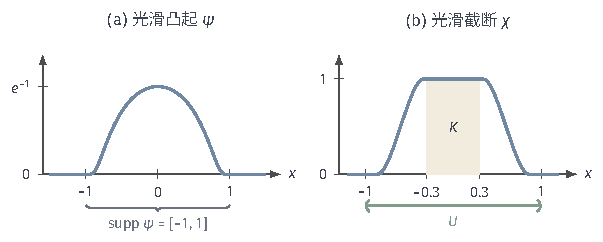
\includegraphics[width=102.2mm]{figures/02-abstract-mathematics/03-function-spaces/tikz/c4-bump-cutoff/figure.pdf}
  \caption{测试函数的两个基本构件。(a)~光滑凸起$\psi$，在$(-1,1)$内为正，在区间外恒为零，各阶导数在$\pm1$处都连续地接到零。(b)~光滑截断$\chi=\mathbf 1_{[-0.6,0.6]}*\rho_{0.3}$：在紧集$K=[-0.3,0.3]$（阴影）上恒为$1$，支撑$[-0.9,0.9]$落在开集$U=(-1,1)$内，中间光滑地由$1$降到$0$。}
  \label{fig:sob-bump-cutoff}
\end{figure}

在$\mathbb R^d$中，把$t^2$换成$|x|^2$就得到在单位开球内为正、在球外为零的光滑凸起$\psi(|x|)$，这里$|x|$是欧氏长度。平移伸缩为$\psi(|x-x_0|/r)$后，它的“非零区域”是以$x_0$为中心、半径为$r$的球。只要$r$小于$x_0$到$\Omega$边界的距离，这个凸起就整个待在$\Omega$内部，离边界还有一段间隔。

\paragraph{支撑与测试函数}
为了把“在边界附近恒为零”说准确，对函数$\varphi$定义它的\term{支撑}（support）
\[
 \operatorname{supp}\varphi=\overline{\{x:\varphi(x)\neq0\}},
\]
即非零点集合的闭包。记$C_c^\infty(\Omega)$为$\Omega$上无穷次可微、且支撑是$\Omega$的紧子集的函数全体，称其中的函数为\term{测试函数}（test function）。支撑紧含于$\Omega$，意味着它与边界保持正距离：存在$\delta>0$，使离边界不到$\delta$的点上$\varphi$恒为零。上面的平移凸起就是测试函数。

这一点立刻解决了分部积分的边界项。设$f\in C^1(\Omega)$，$\varphi\in C_c^\infty(\Omega)$。把$f\varphi$在$\Omega$外补成零，得到$\mathbb R^d$上紧支撑的$C^1$函数。沿第$j$个坐标方向的任一直线积分$\partial_j(f\varphi)$，由微积分基本定理得零，因为两端都落在支撑之外；再对其余坐标积分（Fubini定理~\ref{thm:analysis-fubini-integrable}），得到
\begin{equation}
 \int_\Omega(\partial_jf)\,\varphi\,\mathrm dx=-\int_\Omega f\,\partial_j\varphi\,\mathrm dx .
 \label{eq:sob-integration-by-parts}
\end{equation}
式~\eqref{eq:sob-integration-by-parts}没有边界项，并且右端已不再出现$f$的导数。本章后面的全部构造都从这个等式出发。

\paragraph{局部可积函数}
要让$\int_\Omega f\varphi\,\mathrm dx$有意义，$f$需要满足什么条件？测试函数只在一个紧集上非零，并且在那里有界，所以只需要$f$在每个紧集上可积。称可测函数$f$\term{局部可积}（locally integrable），若对每个紧集$K\subset\Omega$都有$\int_K|f|\,\mathrm dx<\infty$，记作$f\in L^1_{\mathrm{loc}}(\Omega)$；与$L^p$空间一样，几乎处处相等的函数视为同一元素。对$f\in L^1_{\mathrm{loc}}(\Omega)$和支撑在紧集$K$内的测试$\varphi$，
\begin{equation}
 \left|\int_\Omega f\varphi\,\mathrm dx\right|\le\left(\int_K|f|\,\mathrm dx\right)\sup_K|\varphi| ,
 \label{eq:sob-local-pairing}
\end{equation}
右端有限，配对良好定义，而且改变$f$在一个零测集上的值不影响积分。

局部可积比可积宽得多，也依赖于区域。$f(x)=1/x$在$(0,1)$上局部可积：$(0,1)$的紧子集离$0$有正距离，$1/x$在其上有界；但$\int_0^1 x^{-1}\,\mathrm dx=\infty$，所以它不在$L^1(0,1)$中。把区域换成整条实轴，任何含原点的紧区间上积分都发散，$1/x$便不再局部可积。再看$\mathbb R^d$中的幂函数$|x|^{-a}$：按例~\ref{ex:region-power-function-threshold}的二进壳层估计，$d$维壳层$\{2^k\le|x|<2^{k+1}\}$的体积按$2^{kd}$缩放，于是单位球上$\int|x|^{-a}\,\mathrm dx<\infty$当且仅当$a<d$。因此$|x|^{-a}\in L^1_{\mathrm{loc}}(\mathbb R^d)$当且仅当$a<d$。这个阈值在后面检验弱导数和嵌入时会反复使用。

\paragraph{光滑截断}
后面经常需要这样一个测试：它在一个给定紧集上恒等于$1$，又不越出一个给定的开邻域。凸起$\psi$只在一点取最大值，不够用；把它归一化后与示性函数作局部平均，就能得到所需的平台。令$c_d=\int_{\mathbb R^d}\psi(|x|)\,\mathrm dx$，
\begin{equation}
 \rho(x)=c_d^{-1}\psi(|x|),\qquad \rho_\varepsilon(x)=\varepsilon^{-d}\rho(x/\varepsilon)\quad(\varepsilon>0).
 \label{eq:sob-mollifier}
\end{equation}
由换元，$\rho_\varepsilon$非负、光滑、积分为$1$，支撑是闭球$\overline{B}(0,\varepsilon)$。一维时$c_1\approx0.4440$。第~\ref{sec:sob-mollification}节还会把$\rho_\varepsilon$当作局部平均的权重系统使用。

\begin{lemma}[光滑截断]
\label{lem:sob-cutoff}
设$K\subset U\subset\Omega$，$K$紧，$U$开。则存在$\chi\in C_c^\infty(U)$，满足$0\le\chi\le1$，并在$K$上$\chi=1$。
\end{lemma}

\begin{proof}
取$\delta>0$，使$3\delta$小于$K$到$U$的补集的距离（$U=\mathbb R^d$时任取$\delta>0$）；紧集到不相交闭集的距离为正，所以这样的$\delta$存在。记$K_\delta=\{x:\operatorname{dist}(x,K)\le\delta\}$，令
\[
 \chi(x)=\int_{\mathbb R^d}\mathbf 1_{K_\delta}(y)\,\rho_\delta(x-y)\,\mathrm dy .
\]
被积函数对$x$的各阶导数为$\mathbf 1_{K_\delta}(y)D^\alpha\rho_\delta(x-y)$，绝对值不超过$\sup|D^\alpha\rho_\delta|\cdot\mathbf 1_{K_\delta}(y)$，后者与$x$无关且可积，因此可以在积分号下逐次求导（第~\ref{sec:multivariable-parameter-integrals}节），$\chi$无穷次可微。由于$\rho_\delta\ge0$且积分为$1$，有$0\le\chi\le1$。

若$x\in K$，则$\rho_\delta(x-\cdot)$的支撑$\overline B(x,\delta)\subset K_\delta$，积分等于$\int\rho_\delta=1$。若$\operatorname{dist}(x,K)>2\delta$，则$\overline B(x,\delta)$与$K_\delta$不交，$\chi(x)=0$。所以$\operatorname{supp}\chi\subset\{x:\operatorname{dist}(x,K)\le2\delta\}$，这是一个紧集，并且由$\delta$的取法含于$U$。
\end{proof}

图~\ref{fig:sob-bump-cutoff}(b)给出一维的例子：$K=[-0.3,0.3]$，$U=(-1,1)$，取$\delta=0.3$，$\chi=\mathbf 1_{[-0.6,0.6]}*\rho_{0.3}$在$K$上为$1$，在$[-0.9,0.9]$外为零。截断让我们能够“只看一块区域”而不引入跳跃，它在下一节证明测试函数能区分局部可积函数时起关键作用。

\paragraph{测试函数列怎样才算趋零}
广义函数将是测试上的线性读数，我们希望它对测试的小变化作出小反应。那么一列测试$\varphi_n$怎样才算“趋于零”？只看函数值的最大偏差是不够的。图~\ref{fig:sob-test-sequences}比较了三列测试，其中$\psi$为式~\eqref{eq:sob-bump}的凸起。

\begin{figure*}[!htb]
  \centering
  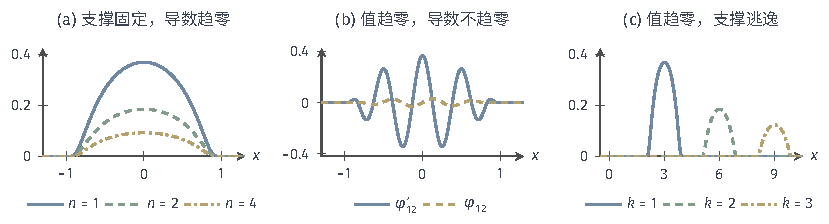
\includegraphics[width=140.4mm]{figures/02-abstract-mathematics/03-function-spaces/tikz/c4-test-sequences/figure.pdf}
  \caption{三列测试函数的对照。(a)~$\psi/n$：支撑固定在$[-1,1]$，函数值及各阶导数都一致趋零，这是测试意义下的趋零。(b)~$\varphi_n=\psi(x)\sin(nx)/n$，图中$n=12$：函数值（虚线）的上确界不超过$e^{-1}/12\approx0.031$，导数（实线）的上确界却约为$e^{-1}\approx0.37$，不随$n$减小。(c)~$\psi(x-3k)/k$：函数值和导数都一致趋零，支撑却跑向无穷远，不落在同一个紧集内。}
  \label{fig:sob-test-sequences}
\end{figure*}

第一列$\psi/n$的支撑固定，每一阶导数都是$D^\alpha\psi/n$，一致趋零；无论用什么合理的方式衡量，它都在变小。第二列$\varphi_n(x)=\psi(x)\sin(nx)/n$的函数值一致趋零，但
\[
 \varphi_n'(x)=\frac{\psi'(x)\sin(nx)}{n}+\psi(x)\cos(nx),
\]
第二项在原点等于$\psi(0)=e^{-1}$，导数并不变小。第三列$\psi(x-3k)/k$的函数值与各阶导数都一致趋零，但支撑向右逃逸，任何固定的紧集都装不下所有项。

后两列在测试意义下都不应算作趋零，因为确实存在合理的读数对它们给出不趋零的结果。读取原点导数的$\varphi\mapsto-\varphi'(0)$在第二列上恒为$-e^{-1}$；读数$\varphi\mapsto\sum_{k\ge1}k\,\varphi(3k)$在每个测试上只有有限项非零，因而有定义，它在第三列的第$k$项上取值$k\cdot\psi(0)/k=e^{-1}$。这两个读数都会在下面被确认为广义函数。于是测试的收敛必须同时控制支撑和所有阶导数：称$\varphi_n\to\varphi$（在测试意义下），若存在同一个紧集$K\subset\Omega$包含所有$\operatorname{supp}\varphi_n$与$\operatorname{supp}\varphi$，并且对每个多重指标$\alpha$都有$\sup_K|D^\alpha\varphi_n-D^\alpha\varphi|\to0$。这里的多重指标约定见第~\ref{sec:sob-distribution-derivative}节；在一维，$D^\alpha$就是$k$阶导数。

这一收敛不是由某一个范数给出的：上确界范数忽略导数，加入有限阶导数也挡不住更高阶的振荡，而支撑条件根本不是范数能表达的。完整的做法是在$C_c^\infty(\Omega)$上建立一种局部凸拓扑，本章不展开这一理论，只使用上面这个序列判据以及下一小节与之配套的估计。

\subsection{广义函数的定义与例子}
\label{sec:sob-distribution-def}

有了测试函数，我们把“对每个测试给出一个数”的对象作为新的研究对象。它应当是线性的，并且在每个固定的紧集上，读数受测试的有限阶导数的大小控制。

\begin{definition}[广义函数]
\label{def:sob-distribution}
称线性映射$T:C_c^\infty(\Omega)\to\mathbb F$为$\Omega$上的\term{广义函数}（generalized function，传统上称distribution），若对每个紧集$K\subset\Omega$，存在常数$C_K\ge0$和非负整数$m_K$，使所有支撑含于$K$的测试$\varphi$满足
\begin{equation}
 |T(\varphi)|\le C_K\sum_{|\alpha|\le m_K}\sup_K|D^\alpha\varphi| .
 \label{eq:sob-distribution-estimate}
\end{equation}
$\Omega$上广义函数的全体记作$\mathcal D'(\Omega)$。
\end{definition}

估计~\eqref{eq:sob-distribution-estimate}保证了上一小节要求的连续性：若$\varphi_n\to\varphi$（测试意义下），所有支撑落在同一个$K$内，对差$\varphi_n-\varphi$用这个估计，右端是有限多个一致趋零的量之和，所以$T(\varphi_n)\to T(\varphi)$。常数$C_K$与阶数$m_K$可以随紧集变化，这让广义函数在区域内部“越靠近边界越剧烈”也被允许。可以证明，反过来序列连续也推出这样的估计，因此两种说法等价；本章只用估计这一侧。广义函数作为线性泛函的观点，与第~\ref{sec:lfo-operators}节对有界线性泛函的讨论一致，区别在于这里的定义域$C_c^\infty(\Omega)$不是赋范空间，连续性只能逐个紧集表述。

\paragraph{由局部可积函数给出的广义函数}
对$f\in L^1_{\mathrm{loc}}(\Omega)$定义
\begin{equation}
 T_f(\varphi)=\int_\Omega f\varphi\,\mathrm dx .
 \label{eq:sob-regular-distribution}
\end{equation}
线性是显然的，估计~\eqref{eq:sob-local-pairing}正是$m_K=0$、$C_K=\int_K|f|$时的式~\eqref{eq:sob-distribution-estimate}，所以$T_f$是广义函数。几乎处处相等的$f$给出同一个$T_f$；下一节将证明反过来也成立，即$T_f=T_g$推出$f=g$几乎处处，于是可以把局部可积函数看作特殊的广义函数而不丢失信息。要强调的是，$T_f$读取的是$f$与测试的加权平均，并没有给$f$补上任何一点处的值：$1/x$在$(0,1)$上产生的广义函数，同样不回答“$f$在某点等于多少”。

\paragraph{点读数与测度}
不由普通函数给出的最简单例子是点读数。固定$x_0\in\Omega$，令
\[
 \delta_{x_0}(\varphi)=\varphi(x_0).
\]
它显然线性，并满足$|\delta_{x_0}(\varphi)|\le\sup_K|\varphi|$，取$m_K=0$、$C_K=1$即可，所以它是广义函数，称为\term{Dirac广义函数}（Dirac delta）。第~\ref{sec:sob-kinks-jumps}节将证明，不存在局部可积函数$g$使$\delta_{x_0}=T_g$。

点读数是测度积分的特例。设$\mu$是$\Omega$上的Borel测度，并且在每个紧集上取有限值（称为局部有限测度），令
\[
 T_\mu(\varphi)=\int_\Omega\varphi\,\mathrm d\mu ,\qquad |T_\mu(\varphi)|\le\mu(K)\sup_K|\varphi| .
\]
它也是$m_K=0$的广义函数。$\delta_{x_0}$对应集中在$x_0$的单位点质量，即第~\ref{sec:lfo-ck-dual}节的Dirac测度；上一小节的读数$\sum_{k\ge1}k\,\varphi(3k)$来自测度$\sum_kk\,\delta_{3k}$，每个紧集只含有限个质点，测度局部有限，所以它也是广义函数；$T_f$在$f\ge0$时对应以$f$为密度的测度$f\,\mathrm dx$，与第~\ref{sec:measure-same-space-comparison}节的Radon--Nikodym密度一致。允许测度带符号（在每个紧集上全变差有限）时，同样的估计以全变差$|\mu|(K)$代替$\mu(K)$。

这样，局部可积函数和局部有限测度都能产生广义函数，但广义函数比它们更宽。它不必是正的：若对所有非负测试都有$T(\varphi)\ge0$，称$T$为正的，$T_f$只在$f\ge0$几乎处处时才正。它也不必由测度给出：由测度给出的广义函数都满足$m_K=0$的估计，只受测试函数值的控制，而下一小节的$D\delta_0$需要读取测试的导数，将越出这一范围。

\subsection{广义函数的微分}
\label{sec:sob-distribution-derivative}

现在可以把导数转移到测试上。先约定多变量的记号。\term{多重指标}（multi-index）是非负整数组$\alpha=(\alpha_1,\ldots,\alpha_d)$，其阶数$|\alpha|=\alpha_1+\cdots+\alpha_d$，对应的偏导数
\[
 D^\alpha=\partial_1^{\alpha_1}\cdots\partial_d^{\alpha_d}.
\]
例如$d=2$、$\alpha=(1,2)$时，$D^\alpha=\partial_1\partial_2^2$，阶数为$3$；$\alpha=(0,\ldots,0)$时约定$D^\alpha$为恒等运算。测试函数的混合偏导数与求导次序无关，因此$D^\alpha$的定义没有歧义。

对$f\in C^{|\alpha|}(\Omega)$和测试$\varphi$，把式~\eqref{eq:sob-integration-by-parts}逐坐标重复$|\alpha|$次，每转移一次导数产生一个负号，测试的紧支撑使每一步都没有边界项：
\begin{equation}
 \int_\Omega(D^\alpha f)\,\varphi\,\mathrm dx=(-1)^{|\alpha|}\int_\Omega f\,D^\alpha\varphi\,\mathrm dx .
 \label{eq:sob-repeated-parts}
\end{equation}
用广义函数的语言，左端是$T_{D^\alpha f}(\varphi)$，右端是$(-1)^{|\alpha|}T_f(D^\alpha\varphi)$。右端对任何广义函数都有意义，于是取它作为定义。

\begin{definition}[广义导数]
\label{def:sob-distribution-derivative}
设$T\in\mathcal D'(\Omega)$，$\alpha$为多重指标。定义$T$的$\alpha$阶\term{广义导数}（distributional derivative）为
\begin{equation}
 (D^\alpha T)(\varphi)=(-1)^{|\alpha|}\,T(D^\alpha\varphi),\qquad\varphi\in C_c^\infty(\Omega).
 \label{eq:sob-distribution-derivative}
\end{equation}
\end{definition}

我们需要核对$D^\alpha T$仍是广义函数。线性由$T$和$D^\alpha$的线性得到。对支撑含于$K$的测试，$D^\alpha\varphi$的支撑也在$K$内，代入$T$的估计，
\[
 |(D^\alpha T)(\varphi)|\le C_K\sum_{|\beta|\le m_K}\sup_K|D^{\beta}D^\alpha\varphi|
 \le C_K\sum_{|\gamma|\le m_K+|\alpha|}\sup_K|D^\gamma\varphi| ,
\]
所以$D^\alpha T$满足阶数为$m_K+|\alpha|$的估计。由此得到三条基本性质。其一，每个广义函数都可以求任意阶导数，导数仍是广义函数，这与经典导数截然不同。其二，由式~\eqref{eq:sob-repeated-parts}，当$f\in C^{|\alpha|}(\Omega)$时$D^\alpha T_f=T_{D^\alpha f}$，新定义与经典导数相容。其三，因为测试的混合偏导数可交换，$D^\alpha D^\beta T=D^{\alpha+\beta}T$，广义导数的次序也无关紧要。

\paragraph{点读数的导数}
看最简单的非函数对象。在实轴上，按定义
\[
 (D\delta_0)(\varphi)=-\delta_0(\varphi')=-\varphi'(0).
\]
$D\delta_0$读取测试在原点的导数并反号，它满足$m_K=1$的估计$|(D\delta_0)(\varphi)|\le\sup_K|\varphi'|$。直观地说，$\delta_0$是集中在原点的单位质量，$D\delta_0$则像在原点两侧紧挨着放置一正一负两个质量所形成的“偶极子”。

$D\delta_0$不能由任何测度给出，下面用固定支撑、函数值有界而原点导数无界的测试来说明。

\begin{example}[$D\delta_0$不是测度]
\label{ex:sob-ddelta-not-measure}
设有实轴上的带符号Borel测度$\mu$，在紧集上全变差有限，并且$D\delta_0=T_\mu$。取光滑截断$\chi$，使其在$[-0.3,0.3]$上为$1$、支撑在$[-0.9,0.9]$内（例如图~\ref{fig:sob-bump-cutoff}(b)中的函数），令
\[
 \varphi_n(x)=\chi(x)\sin(nx).
\]
每个$\varphi_n$的支撑都在$K=[-0.9,0.9]$内，且$|\varphi_n|\le1$。由于$\chi$在原点附近恒为$1$，$\varphi_n'(0)=n\cos0=n$。一方面$|T_\mu(\varphi_n)|\le|\mu|(K)\sup|\varphi_n|\le|\mu|(K)$；另一方面$|(D\delta_0)(\varphi_n)|=|\varphi_n'(0)|=n$。令$n\to\infty$即得矛盾。图~\ref{fig:sob-ddelta-test}画出$n=3$与$n=10$的测试及其原点切线。
\end{example}

\begin{figure}[!htb]
  \centering
  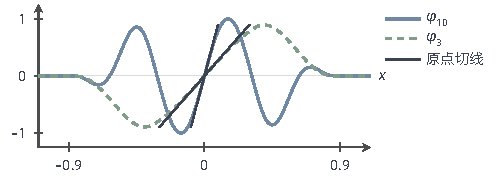
\includegraphics[width=84.4mm]{figures/02-abstract-mathematics/03-function-spaces/tikz/c4-ddelta-test/figure.pdf}
  \caption{区分$D\delta_0$与测度的测试$\varphi_n(x)=\chi(x)\sin(nx)$，$n=3$（虚线）与$n=10$（实线）。两者的支撑都在$[-0.9,0.9]$内，函数值都不超过$1$，测度的读数因而一致有界；原点处的切线斜率却等于$n$，$D\delta_0$的读数$-\varphi_n'(0)=-n$随$n$无界。}
  \label{fig:sob-ddelta-test}
\end{figure}

这个例子与上一小节图~\ref{fig:sob-test-sequences}(b)是同一个机制：只控制函数值不能控制导数的读数。它说明广义函数严格大于测度，求导会把函数（甚至测度）推出原来的对象类型。于是自然要问：从一个局部可积函数出发，它的广义导数什么时候仍然是一个局部可积函数？这正是下一节要回答的问题。

% 第4章第2节：弱导数与经典微分（弱导数的定义与唯一性、尖点跳跃与奇异变化、一维弱导数与绝对连续性）。

\section{弱导数与经典微分}
\label{sec:sob-weak-derivatives}

上一节说明，任何局部可积函数$f$都有各阶广义导数$D^\alpha T_f$，但它们可能是$\delta_0$这样的点读数，甚至连测度都不是。本节固定$f\in L^1_{\mathrm{loc}}(\Omega)$，研究一个更具体的问题：$D^\alpha T_f$什么时候仍由一个局部可积函数给出。我们先给出定义并证明这样的函数在几乎处处意义下唯一，再用尖点、跳跃和Cantor函数比较三种不同的结局，最后在一维情形证明，这个条件恰好等价于函数有绝对连续的代表。

\subsection{弱导数的定义与唯一性}
\label{sec:sob-weak-derivative-def}

若广义导数$D^\alpha T_f$等于某个$T_g$，按式~\eqref{eq:sob-distribution-derivative}与式~\eqref{eq:sob-regular-distribution}展开，就是对所有测试成立一个积分恒等式。我们把这个恒等式直接作为定义。

\begin{definition}[弱导数]
\label{def:sob-weak-derivative}
设$f,g\in L^1_{\mathrm{loc}}(\Omega)$，$\alpha$为多重指标。若对所有$\varphi\in C_c^\infty(\Omega)$都有
\begin{equation}
 \int_\Omega g\,\varphi\,\mathrm dx=(-1)^{|\alpha|}\int_\Omega f\,D^\alpha\varphi\,\mathrm dx ,
 \label{eq:sob-weak-derivative}
\end{equation}
则称$g$为$f$的$\alpha$阶\term{弱导数}（weak derivative），记作$D^\alpha f=g$。一阶情形也写作$\partial_jf$，全部一阶弱导数组成的向量记作弱梯度$\nabla f$。
\end{definition}

与广义导数相比，这里多了一个实质性的条件：存在一个局部可积函数$g$来表示$D^\alpha T_f$。广义导数总存在，弱导数却未必。恒等式必须对\emph{所有}测试成立，只在若干个测试上核对是不够的；也不能用“经典导数几乎处处存在”来代替它，第~\ref{sec:sob-kinks-jumps}节的阶跃和Cantor函数会说明这一点。由式~\eqref{eq:sob-repeated-parts}，$C^{|\alpha|}$函数的经典导数就是弱导数，所以这一定义推广了经典导数。

\paragraph{运算规则}
弱导数对$f$是线性的：若$D^\alpha f_1=g_1$，$D^\alpha f_2=g_2$，则对标量$a,b$有$D^\alpha(af_1+bf_2)=ag_1+bg_2$，因为恒等式~\eqref{eq:sob-weak-derivative}两边都对$f$和$g$线性。与光滑函数相乘也有乘积法则。设$a\in C^\infty(\Omega)$，$f$有一阶弱导数$\partial_jf$。对任意测试$\varphi$，$a\varphi$仍是测试，且$\partial_j(a\varphi)=a\,\partial_j\varphi+\varphi\,\partial_ja$，于是
\[
 \int_\Omega af\,\partial_j\varphi\,\mathrm dx
 =\int_\Omega f\,\partial_j(a\varphi)\,\mathrm dx-\int_\Omega f\varphi\,\partial_ja\,\mathrm dx
 =-\int_\Omega\bigl(a\,\partial_jf+f\,\partial_ja\bigr)\varphi\,\mathrm dx ,
\]
第二个等号对测试$a\varphi$使用了弱导数的定义。右端括号内的函数局部可积，所以$\partial_j(af)=a\,\partial_jf+f\,\partial_ja$。

两个都弱可微的函数相乘则要另查可积性。在$\mathbb R^3$中取$f(x)=|x|^{-6/5}$。它在原点外光滑，$|\nabla f|=\frac65|x|^{-11/5}$；由上一节的幂函数阈值，$f$与$|\nabla f|$都局部可积（$6/5<3$，$11/5<3$），用挖去小球再令半径趋零的分部积分可以验证$\nabla f$确实是弱梯度。可是乘积法则给出的候选$2f\nabla f$大小为$\frac{12}{5}|x|^{-17/5}$，指数$17/5>3$，不局部可积。因此$f^2=|x|^{-12/5}$虽然局部可积，却没有局部可积的弱梯度。乘积法则只在各项可积时才能使用。

\paragraph{测试函数区分局部可积函数}
为了说明弱导数确定到几乎处处，我们先证明一条更基本的事实：如果一个局部可积函数与所有测试的配对都为零，它本身几乎处处为零。证明需要Lebesgue测度的两条正则性：对正测度的可测集$A$，存在紧集$C\subset A$且$|C|>0$（内正则性）；对任意可测集$C$和$\eta>0$，存在开集$U\supset C$使$|U\setminus C|<\eta$（外正则性）。这里$|\cdot|$表示Lebesgue测度。外正则性来自用可数个开盒子覆盖来定义Lebesgue外测度的方式，内正则性可由外正则性对补集使用得到。证明还要用到积分的绝对连续性：若$h$在集合$E_0$上可积，则对任意$\eta>0$，存在$\delta>0$，使$E_0$中测度小于$\delta$的子集$E$都满足$\int_E|h|<\eta$。

\begin{lemma}[测试函数区分局部可积函数]
\label{lem:sob-fundamental}
设$h\in L^1_{\mathrm{loc}}(\Omega)$，且对所有$\varphi\in C_c^\infty(\Omega)$都有$\int_\Omega h\varphi\,\mathrm dx=0$。则$h=0$几乎处处。
\end{lemma}

\begin{proof}
复值时分别处理实部和虚部（实值测试的配对分别给出两者的配对），所以只需考虑实值$h$。反设$h$不几乎处处为零，则$\{h>0\}$或$\{h<0\}$有正测度；以$-h$代替$h$，不妨设$\{h>0\}$有正测度。

第一步，找一块有正积分的紧集。令$G_m=\{x\in\Omega:|x|<m,\ \operatorname{dist}(x,\partial\Omega)>1/m\}$（$\Omega=\mathbb R^d$时只要求$|x|<m$），它们是递增的开集，闭包紧且含于$\Omega$，并集为$\Omega$。由可数可加性，某个$A=\{h>0\}\cap G_m$有正测度。内正则性给出紧集$C\subset A$且$|C|>0$；$h$在$C$上为正，所以$a:=\int_Ch\,\mathrm dx>0$。

第二步，用截断控制外侧误差。$h$在紧集$\overline{G_{m+1}}$上可积，由积分的绝对连续性，取$\delta>0$使$\overline{G_{m+1}}$中测度小于$\delta$的集合$E$满足$\int_E|h|<a/2$。外正则性给出开集$U'\supset C$且$|U'\setminus C|<\delta$；令$U=U'\cap G_{m+1}$，它仍是包含$C$的开集。由引理~\ref{lem:sob-cutoff}，取$\chi\in C_c^\infty(U)$，$0\le\chi\le1$，在$C$上$\chi=1$。

第三步，计算配对。因为$\chi$在$C$上为$1$，在$U$外为$0$，
\[
 \int_\Omega h\chi\,\mathrm dx=\int_Ch\,\mathrm dx+\int_{U\setminus C}h\chi\,\mathrm dx
 \ge a-\int_{U\setminus C}|h|\,\mathrm dx>a-\frac a2>0 ,
\]
与假设$\int h\chi=0$矛盾。所以$h=0$几乎处处。
\end{proof}

这条引理的证明只用了截断函数和测度的正则性，没有借助后面的平滑逼近定理。它的作用是说明：测试函数足够多，能够把局部可积函数的等价类彼此分开。直接的推论是映射$f\mapsto T_f$是单射：$T_f=T_g$意味着$f-g$与所有测试的配对为零，从而$f=g$几乎处处。

\begin{theorem}[弱导数的唯一性]
\label{thm:sob-weak-derivative-unique}
设$f\in L^1_{\mathrm{loc}}(\Omega)$。若$g_1,g_2\in L^1_{\mathrm{loc}}(\Omega)$都是$f$的$\alpha$阶弱导数，则$g_1=g_2$几乎处处。
\end{theorem}

\begin{proof}
两个恒等式~\eqref{eq:sob-weak-derivative}的右端相同，相减得$\int(g_1-g_2)\varphi=0$对所有测试成立，由引理~\ref{lem:sob-fundamental}即得结论。
\end{proof}

唯一的是等价类：改变$g$在零测集上的值不破坏恒等式，所以“弱导数在某一点的值”没有意义，正如$L^p$元素在一点的值没有意义一样。

\subsection{尖点、跳跃与奇异变化}
\label{sec:sob-kinks-jumps}

现在比较三个在单点或零测集上“出问题”的函数。它们都几乎处处有经典导数，却分别落在三种不同的结局里。

\paragraph{尖点：$|x|$}
在实轴上取$f(x)=|x|$。对测试$\varphi$，在原点两侧分别分部积分：
\[
\begin{aligned}
 \int_{-\infty}^{\infty}|x|\varphi'(x)\,\mathrm dx
 &=\int_{-\infty}^0(-x)\varphi'(x)\,\mathrm dx+\int_0^\infty x\varphi'(x)\,\mathrm dx\\
 &=\Bigl[-x\varphi(x)\Bigr]_{-\infty}^{0}+\int_{-\infty}^0\varphi\,\mathrm dx
 +\Bigl[x\varphi(x)\Bigr]_{0}^{\infty}-\int_0^\infty\varphi\,\mathrm dx\\
 &=-\int_{-\infty}^{\infty}\operatorname{sgn}(x)\,\varphi(x)\,\mathrm dx .
\end{aligned}
\]
四个边界项都为零：在$\pm\infty$一侧，测试紧支撑；在原点一侧，因子$x$等于零。这正是式~\eqref{eq:sob-weak-derivative}在$\alpha=1$、$g=\operatorname{sgn}x$时的形式，所以$|x|$的弱导数是$\operatorname{sgn}x$（图~\ref{fig:sob-abs-sign}）。原点的经典导数不存在，但这只涉及一个零测点；$\operatorname{sgn}0$取什么值都不影响结论。

\begin{figure}[!htb]
  \centering
  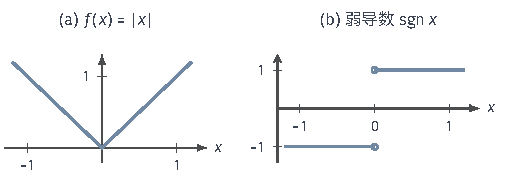
\includegraphics[width=85.7mm]{figures/02-abstract-mathematics/03-function-spaces/tikz/c4-abs-sign/figure.pdf}
  \caption{尖点函数与它的弱导数。(a)~$f(x)=|x|$在原点连续但有尖点；(b)~弱导数$\operatorname{sgn}x$在原点两侧分别为$-1$与$1$，空心点表示原点的取值可以任意约定，弱导数作为等价类不受影响。}
  \label{fig:sob-abs-sign}
\end{figure}

边界项在原点相消，靠的是$|x|$在原点连续。下面的阶跃函数在原点断开，同样的计算会留下一个点读数。

\paragraph{跳跃：阶跃函数}
取$H=\mathbf 1_{(0,\infty)}$。对测试$\varphi$，
\[
 (DT_H)(\varphi)=-\int_{-\infty}^{\infty}H\varphi'\,\mathrm dx=-\int_0^\infty\varphi'\,\mathrm dx=\varphi(0),
\]
所以$DT_H=\delta_0$。$H$在原点外处处可导且经典导数为零，但零函数不是它的弱导数：$\int0\cdot\varphi=0$，而$\delta_0(\varphi)=\varphi(0)$对$\varphi(0)\neq0$的测试不为零。跳跃把变化全部集中在一点上，留下的是测试在跳点的取值。

还要说明$\delta_0$不能由\emph{任何}局部可积函数表示，这样$H$才确实没有弱导数。

\begin{example}[$\delta_0$不是局部可积函数]
\label{ex:sob-delta-not-function}
反设$g\in L^1_{\mathrm{loc}}(\mathbb R)$使$\delta_0=T_g$。取图~\ref{fig:sob-bump-cutoff}(b)中的截断$\chi$，令$\varphi_\varepsilon(x)=\chi(x/\varepsilon)$，$0<\varepsilon\le1$。每个$\varphi_\varepsilon$满足$0\le\varphi_\varepsilon\le1$、$\varphi_\varepsilon(0)=1$，支撑在$[-\varepsilon,\varepsilon]$内（图~\ref{fig:sob-step-delta}(b)）。于是
\[
 1=\delta_0(\varphi_\varepsilon)=\int g\varphi_\varepsilon\,\mathrm dx,\qquad
 \left|\int g\varphi_\varepsilon\,\mathrm dx\right|\le\int_{-\varepsilon}^{\varepsilon}|g|\,\mathrm dx .
\]
$g$在$[-1,1]$上可积，区间$[-\varepsilon,\varepsilon]$的测度趋于零，由积分的绝对连续性，右端趋于零，与左端恒为$1$矛盾。
\end{example}

\begin{figure}[!htb]
  \centering
  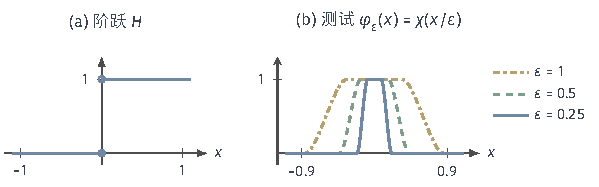
\includegraphics[width=101.5mm]{figures/02-abstract-mathematics/03-function-spaces/tikz/c4-step-delta/figure.pdf}
  \caption{跳跃留下点读数。(a)~阶跃$H=\mathbf 1_{(0,\infty)}$，其广义导数为$\delta_0$。(b)~支撑缩小的测试$\varphi_\varepsilon(x)=\chi(x/\varepsilon)$，$\varepsilon=1,0.5,0.25$：原点值始终为$1$，因此$\delta_0$的读数恒为$1$；而任何局部可积函数与$\varphi_\varepsilon$的配对都被它在越来越短区间上的积分控制，趋于零。}
  \label{fig:sob-step-delta}
\end{figure}

图~\ref{fig:sob-step-delta}把两种读数的差别画了出来：点读数只看原点，测试缩得再窄，读数也不变；函数的积分读数却要乘上支撑的宽度，最终消失。顺带可知$\operatorname{sgn}x=2H-1$的广义导数是$2\delta_0$，所以$|x|$有一阶弱导数，却没有二阶弱导数。

\paragraph{奇异连续变化：Cantor函数}
跳跃的变化集中在一点，函数因而不连续。是否连续函数、且经典导数几乎处处存在，就一定有弱导数？Cantor函数给出否定的回答。

回顾它的构造。从$[0,1]$出发，挖去中间三分之一的开区间$(1/3,2/3)$，在其上令$c=1/2$；对剩下的两个闭区间各自挖去中间三分之一，在$(1/9,2/9)$上令$c=1/4$，在$(7/9,8/9)$上令$c=3/4$；如此继续，第$m$步挖去$2^{m-1}$个长为$3^{-m}$的开区间，并在其上分别取相邻两层平台值的平均。被挖去区间的总长度为$\sum_{m\ge1}2^{m-1}3^{-m}=1$，剩下的Cantor集测度为零。再令$c(0)=0$、$c(1)=1$，并在Cantor集上按单调性补齐，得到$[0,1]$上连续、单调不减的函数$c$（图~\ref{fig:sob-cantor}(a)）。它在每个被挖去的开区间上为常数，所以在测度为$1$的集合上经典导数为零。以概率的语言说，$c$是一个随机变量的分布函数，这个随机变量没有任何单点概率，也没有密度；这一观察可参考\BookChapterRef{chap:random-variables}{卷一“随机变量与概率分布”章}。

\begin{figure}[!htb]
  \centering
  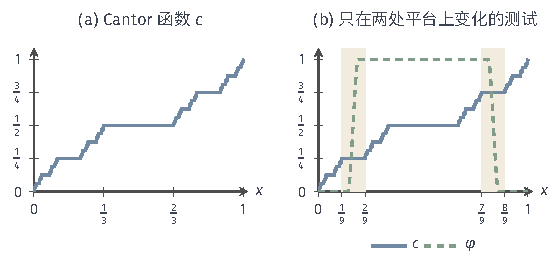
\includegraphics[width=94.7mm]{figures/02-abstract-mathematics/03-function-spaces/tikz/c4-cantor/figure.pdf}
  \caption{Cantor函数没有弱导数。(a)~$c$连续、单调，在被挖去的区间$(\frac13,\frac23)$、$(\frac19,\frac29)$、$(\frac79,\frac89)$等上为常数，在测度为$1$的集合上经典导数为零。(b)~测试$\varphi$（虚线）只在阴影区间$(\frac19,\frac29)$与$(\frac79,\frac89)$内变化，那里$c$分别为$\frac14$与$\frac34$，于是$-\int c\varphi'=-\frac14+\frac34=\frac12$；若$c$有弱导数，这个读数必须为零。}
  \label{fig:sob-cantor}
\end{figure}

\begin{example}[Cantor函数没有弱导数]
\label{ex:sob-cantor}
反设$c$在$(0,1)$上有弱导数$g\in L^1_{\mathrm{loc}}(0,1)$。先在每个被挖去的开区间$I$上看：对支撑在$I$内的测试$\varphi$，$c$在$I$上为常数$c_I$，所以
\[
 \int_Ig\varphi\,\mathrm dx=-\int_Ic_I\,\varphi'\,\mathrm dx=0 .
\]
对开集$I$使用引理~\ref{lem:sob-fundamental}，得$g=0$在$I$上几乎处处成立。被挖去的区间可数个，总长为$1$，因此$g=0$在$(0,1)$上几乎处处成立，从而对所有测试都应有$\int c\varphi'=-\int g\varphi=0$。

再取一个具体测试：$\varphi$在$(1/9,2/9)$内由$0$光滑地升到$1$，在$[2/9,7/9]$上恒为$1$，在$(7/9,8/9)$内光滑地降到$0$（图~\ref{fig:sob-cantor}(b)）。$\varphi'$只在这两个区间内非零，而$c$在那里分别等于$1/4$和$3/4$，所以
\[
 \begin{aligned}
 -\int_0^1c\,\varphi'\,\mathrm dx
 &=-\frac14\int_{1/9}^{2/9}\varphi'\,\mathrm dx-\frac34\int_{7/9}^{8/9}\varphi'\,\mathrm dx\\
 &=-\frac14\cdot1-\frac34\cdot(-1)=\frac12\neq0 ,
 \end{aligned}
\]
矛盾。所以$c$没有弱导数。
\end{example}

读数$1/2$正好是$c$在$[2/9,7/9]$上的增量。实际上，$c$的广义导数是$c$所对应的Lebesgue--Stieltjes测度$\mu_c$（由$\mu_c((s,t])=c(t)-c(s)$确定），它集中在测度为零的Cantor集上，相对Lebesgue测度是奇异的；按第~\ref{sec:measure-lebesgue-decomposition}节的Lebesgue分解（定理~\ref{thm:measure-lebesgue-decomposition}），它没有绝对连续部分，因而不能写成$g\,\mathrm dx$。

\paragraph{三个例子的对照}
表~\ref{tab:sob-three-examples}把三个函数放在一起。三者都几乎处处有经典导数，广义导数也都存在，区别在于广义导数是什么类型的对象。只有$|x|$的广义导数是局部可积函数，才有弱导数；阶跃的变化集中成点质量，Cantor函数的变化集中成奇异连续测度。所以“几乎处处可微”与“弱可微”是两回事：前者只看测度为$1$的集合上的局部斜率，后者要求整体的积分恒等式成立。

\begin{table}[!htb]
 \centering
 \caption{尖点、跳跃与奇异连续变化的对照（区间$(-1,1)$或$(0,1)$上）。}
 \label{tab:sob-three-examples}
 \begin{tabular}{@{}llll@{}}
  \toprule
  函数 & 经典导数 & 广义导数 & 有无弱导数\\
  \midrule
  $|x|$ & 除原点外为$\operatorname{sgn}x$ & $T_{\operatorname{sgn}}$ & 有，$\operatorname{sgn}x$\\
  $H=\mathbf 1_{(0,\infty)}$ & 除原点外为$0$ & $\delta_0$ & 无\\
  Cantor函数$c$ & 几乎处处为$0$ & 奇异测度$\mu_c$ & 无\\
  \bottomrule
 \end{tabular}
\end{table}

$|x|$与另两者的差别在于，它能由自己的导数积分恢复：$|x|=|x_0|+\int_{x_0}^x\operatorname{sgn}t\,\mathrm dt$。阶跃和Cantor函数都做不到这一点，因为它们的经典导数积分出来恒为零。下一小节证明，在一维情形，“能由导数积分恢复”恰好就是弱可微的含义。

\subsection{一维弱导数与绝对连续性}
\label{sec:sob-absolute-continuity}

本小节在有限区间$(a,b)$上工作，记长度$L=b-a$。我们先证明弱导数为零的函数是常数，再借此把弱导数与积分表示联系起来。

\begin{lemma}[弱导数为零的函数]
\label{lem:sob-zero-derivative}
设$f\in L^1_{\mathrm{loc}}(a,b)$，且$\int_a^bf\varphi'\,\mathrm dx=0$对所有$\varphi\in C_c^\infty(a,b)$成立。则存在常数$c$，使$f=c$几乎处处。
\end{lemma}

\begin{proof}
关键是看出哪些测试能写成另一个测试的导数。若$\psi\in C_c^\infty(a,b)$且$\int\psi=0$，则$\varphi(x)=\int_a^x\psi(t)\,\mathrm dt$是光滑的；在$\operatorname{supp}\psi$左侧$\varphi=0$，在其右侧$\varphi=\int\psi=0$，所以$\varphi\in C_c^\infty(a,b)$且$\varphi'=\psi$。于是假设给出：$f$与每个积分为零的测试配对为零。

固定一个积分为$1$的测试$\theta$（例如平移伸缩后的$\rho_\varepsilon$）。任意测试$\psi$可写成$\psi=\bigl(\int\psi\bigr)\theta+\bigl(\psi-(\int\psi)\theta\bigr)$，后一项积分为零，与$f$的配对为零。所以
\[
 \int_a^bf\psi\,\mathrm dx=\Bigl(\int_a^b\psi\,\mathrm dx\Bigr)\int_a^bf\theta\,\mathrm dx=\int_a^bc\,\psi\,\mathrm dx,\qquad c=\int_a^bf\theta\,\mathrm dx .
\]
即$f-c$与所有测试的配对为零，由引理~\ref{lem:sob-fundamental}，$f=c$几乎处处。
\end{proof}

接下来需要一维实分析中的绝对连续函数。称$F:[a,b]\to\mathbb F$\term{绝对连续}（absolutely continuous），若对任意$\varepsilon>0$存在$\delta>0$，使对$[a,b]$中任意有限个两两不交的子区间$(x_i,y_i)$，只要$\sum_i(y_i-x_i)<\delta$，就有$\sum_i|F(y_i)-F(x_i)|<\varepsilon$。它比一致连续强：一致连续只控制一个短区间上的增量，绝对连续控制总长度很短的许多区间上增量之和。Cantor函数连续却不绝对连续：第$m$步剩下$2^m$个闭区间，总长$(2/3)^m$可以任意小，$c$在它们上的增量之和却始终为$1$。

下面使用Lebesgue关于绝对连续函数的微积分基本定理，不在这里证明：若$g\in L^1(a,b)$，则$G(x)=\int_a^xg(t)\,\mathrm dt$在$[a,b]$上绝对连续，且$G'=g$几乎处处；反过来，若$F$在$[a,b]$上绝对连续，则$F$几乎处处可导，$F'\in L^1(a,b)$，并且$F(x)=F(a)+\int_a^xF'(t)\,\mathrm dt$。当$F$单调不减时，这正是说$F$对应的Lebesgue--Stieltjes测度相对Lebesgue测度绝对连续，$F'$是Radon--Nikodym密度（定理~\ref{thm:density-radon-nikodym}）；Cantor函数的测度则完全奇异。

\begin{theorem}[一维弱导数与绝对连续代表]
\label{thm:sob-1d-absolute-continuity}
设$f,g\in L^1(a,b)$。则$g$是$f$的弱导数，当且仅当$f$有一个绝对连续的代表$\tilde f$，满足
\begin{equation}
 \tilde f(y)-\tilde f(x)=\int_x^yg(t)\,\mathrm dt,\qquad a\le x\le y\le b .
 \label{eq:sob-1d-integral-representation}
\end{equation}
此时$\tilde f$在$[a,b]$上唯一，几乎处处有经典导数$\tilde f'=g$。
\end{theorem}

\begin{proof}
先证明累积积分$G(x)=\int_a^xg(t)\,\mathrm dt$以$g$为弱导数。对测试$\varphi$，
\[
 \begin{aligned}
 \int_a^bG\varphi'\,\mathrm dx&=\int_a^b\!\!\int_a^b\mathbf 1_{\{t<x\}}\,g(t)\varphi'(x)\,\mathrm dt\,\mathrm dx\\
 &=\int_a^bg(t)\Bigl(\int_t^b\varphi'(x)\,\mathrm dx\Bigr)\mathrm dt=-\int_a^bg\varphi\,\mathrm dt .
 \end{aligned}
\]
交换积分次序的依据是Fubini定理：被积函数的绝对值不超过$|g(t)|\sup|\varphi'|$，在正方形$[a,b]^2$上可积。最后一步用了$\varphi(b)=0$。

必要性。若$g$是$f$的弱导数，则$f-G$的弱导数为零，由引理~\ref{lem:sob-zero-derivative}，存在常数$c$使$f=c+G$几乎处处。$\tilde f=c+G$绝对连续，并满足式~\eqref{eq:sob-1d-integral-representation}。

充分性。若$f$有满足式~\eqref{eq:sob-1d-integral-representation}的代表，取$x=a$得$\tilde f=\tilde f(a)+G$，常数的弱导数为零，所以$f$的弱导数就是$G$的弱导数$g$。

唯一性：两个连续代表几乎处处相等，在区间的每个非空开子集上不可能处处不同，因而处处相等（非空开区间的Lebesgue测度为正）。$\tilde f'=g$几乎处处来自上面引用的Lebesgue定理。
\end{proof}

定理把一维弱可微性完全翻译成了经典语言：有弱导数，就是能从导数积分回来。把条件放宽到$f,g\in L^1_{\mathrm{loc}}(a,b)$时，同样的论证给出一个在每个紧子区间上绝对连续的代表，只是它可能在端点附近无界，例如$(0,1)$上$f(x)=\ln x$，弱导数$1/x$局部可积但不可积。

\paragraph{积分指数给出Hölder控制}
若进一步知道$g\in L^p(a,b)$，式~\eqref{eq:sob-1d-integral-representation}还能定量地控制$\tilde f$的振荡。对$1<p<\infty$，设$q$为共轭指数，$1/p+1/q=1$。由Hölder不等式，
\begin{equation}
 |\tilde f(y)-\tilde f(x)|\le\int_x^y|g|\cdot1\,\mathrm dt\le\|g\|_{L^p}\,|y-x|^{1/q}=\|g\|_{L^p}\,|y-x|^{1-1/p} .
 \label{eq:sob-1d-holder}
\end{equation}
称满足$|F(x)-F(y)|\le M|x-y|^\gamma$的函数为$\gamma$阶\term{Hölder连续}（Hölder continuous），$0<\gamma\le1$；$\gamma=1$即Lipschitz连续。式~\eqref{eq:sob-1d-holder}说明$\tilde f$是$1-1/p$阶Hölder连续的，指数随$p$增大而增大；$p=\infty$时直接得到Lipschitz控制$|\tilde f(y)-\tilde f(x)|\le\|g\|_{L^\infty}|y-x|$。图~\ref{fig:sob-holder-1d}(a)画出了几种控制函数$h^{1-1/p}$。

\begin{figure}[!htb]
  \centering
  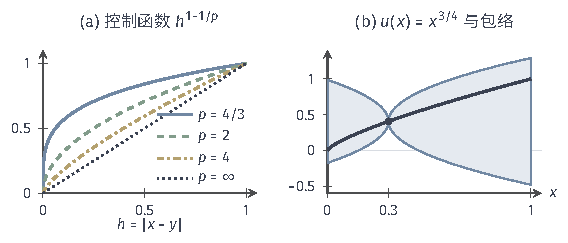
\includegraphics[width=96.2mm]{figures/02-abstract-mathematics/03-function-spaces/tikz/c4-holder-1d/figure.pdf}
  \caption{导数的积分指数控制函数的振荡。(a)~控制函数$h^{1-1/p}$，$p=4/3,2,4,\infty$对应Hölder指数$\frac14,\frac12,\frac34,1$；指数越小，短距离上允许的变化越大。(b)~$u(x)=x^{3/4}$的弱导数$\frac34x^{-1/4}$属于$L^2(0,1)$，$\|u'\|_{L^2}=\sqrt{9/8}\approx1.061$；由式~\eqref{eq:sob-1d-holder}，$u$的图像必须留在以$(0.3,u(0.3))$为顶点的阴影包络$u(0.3)\pm1.061|x-0.3|^{1/2}$内。}
  \label{fig:sob-holder-1d}
\end{figure}

图~\ref{fig:sob-holder-1d}(b)用一个具体函数检验这一估计。$u(x)=x^{3/4}$在原点的经典导数无界，但$u'(x)=\frac34x^{-1/4}$满足$\int_0^1|u'|^2=\frac9{16}\int_0^1x^{-1/2}\,\mathrm dx=\frac98$，所以$u'\in L^2(0,1)$；按定理~\ref{thm:sob-1d-absolute-continuity}它就是弱导数。取$p=2$，式~\eqref{eq:sob-1d-holder}说明$u$的图像整条落在以任一点为顶点、开口为$\sqrt{9/8}\,|x-y|^{1/2}$的包络内，图中以$y=0.3$为例。

$p=1$是例外：此时仍有绝对连续代表，却没有任何正的Hölder指数保证。例如在$(0,1/2)$上取$f(x)=1/\ln(1/x)$，并令$f(0)=0$。它单调增加，$f'(x)=1/\bigl(x\ln^2(1/x)\bigr)$，$\int_0^{1/2}f'=f(1/2)-f(0^+)=1/\ln2$有限，所以$f'\in L^1$。但对任意$\gamma>0$，$h^\gamma\ln(1/h)\to0$（$h\to0^+$），即$f(h)-f(0)=1/\ln(1/h)$比$h^\gamma$大得多，$f$在原点不满足任何正阶Hölder条件。

\paragraph{点值与端点值}
上面的估计还给出用$L^p$大小控制点值的方法。设$f,g\in L^p(a,b)$，$1\le p<\infty$。若$|\tilde f|$处处大于$L^{-1/p}\|f\|_{L^p}$，则$\int|\tilde f|^p>L\cdot L^{-1}\|f\|_{L^p}^p$，矛盾；所以存在$y\in[a,b]$使$|\tilde f(y)|\le L^{-1/p}\|f\|_{L^p}$。对任意$x\in[a,b]$，再由式~\eqref{eq:sob-1d-holder}（$p=1$时直接用$\int|g|$），
\begin{equation}
 \sup_{x\in[a,b]}|\tilde f(x)|\le L^{-1/p}\|f\|_{L^p}+L^{1-1/p}\|g\|_{L^p} .
 \label{eq:sob-1d-sup-bound}
\end{equation}
$p=2$时右端是$L^{-1/2}\|f\|_{L^2}+L^{1/2}\|g\|_{L^2}$。这个估计对闭区间的每一点同时成立，端点也包括在内。

要强调的是，这里的点值都是指唯一的连续代表$\tilde f$的值。在等价类中任取另一个代表，它可以在任意一个零测集上改值，点值便失去意义；正是弱导数的存在，从等价类中选出了唯一一个连续成员。这一结论依赖于一维：在高维，即使函数和全部一阶弱导数都平方可积，函数也可能在一点附近无界，第~\ref{sec:sob-embedding}节将看到维数和积分指数怎样共同决定连续代表是否存在。

% 第4章第3节：Sobolev空间（成员条件与范数、弱微分的定义域、完备性与Hilbert结构）。

\section{Sobolev空间}
\label{sec:sob-spaces}

弱导数的存在只回答了输出是什么类型的对象，还没有限制函数和导数有多大。$|x|$在整条实轴上有弱导数$\operatorname{sgn}x$，可两者都不可积；$\sin(nx)$的导数是$n\cos(nx)$，函数大小不变而导数随$n$无界。要把“变化受控”变成可以计算误差、取极限的条件，需要把函数和它的各阶弱导数一起放进范数。本节建立这样的空间，并证明极限过程中导数关系不会丢失。

\subsection{成员条件与Sobolev范数}
\label{sec:sob-norms}

我们希望同时控制函数本身和它直到某一阶的全部弱导数，并以$L^p$范数衡量每一项。

\begin{definition}[Sobolev空间]
\label{def:sob-sobolev-space}
设$\Omega\subset\mathbb R^d$为开集，$k\ge0$为整数，$1\le p<\infty$。称
\[
 W^{k,p}(\Omega)=\bigl\{u\in L^p(\Omega):\ \text{对每个}|\alpha|\le k,\ D^\alpha u\text{ 存在且属于 }L^p(\Omega)\bigr\}
\]
为\term{Sobolev空间}（Sobolev space），其中$D^0u=u$，并赋以\term{Sobolev范数}（Sobolev norm）
\begin{equation}
 \|u\|_{W^{k,p}}=\Bigl(\sum_{|\alpha|\le k}\|D^\alpha u\|_{L^p}^p\Bigr)^{1/p} .
 \label{eq:sob-sobolev-norm}
\end{equation}
\end{definition}

这里的元素仍是几乎处处等价类，各阶弱导数由定理~\ref{thm:sob-weak-derivative-unique}确定到几乎处处。$L^p(\Omega)$的函数在每个紧集上可积（在紧集$K$上由Hölder不等式，$\int_K|u|\le|K|^{1-1/p}\|u\|_{L^p}$），所以定义中的弱导数恒等式都有意义。范数~\eqref{eq:sob-sobolev-norm}是有限个$L^p$范数的$\ell^p$组合：齐次性显然；三角不等式先对每个分量用$L^p$的Minkowski不等式，再对有限维向量$(\|D^\alpha u\|_{L^p})_\alpha$用$\ell^p$的Minkowski不等式；若$\|u\|_{W^{k,p}}=0$，则零阶项$\|u\|_{L^p}=0$，$u=0$。$k=0$时$W^{0,p}=L^p$。

\paragraph{用前面的例子检验成员条件}
在区间$(-1,1)$上，$|x|$和$\operatorname{sgn}x$都属于$L^p$，而$\operatorname{sgn}x$就是$|x|$的弱导数，所以$|x|\in W^{1,p}(-1,1)$对每个$1\le p<\infty$成立。直接计算$\|\,|x|\,\|_{L^p}^p=2/(p+1)$，$\|\operatorname{sgn}\|_{L^p}^p=2$，于是
\[
 \|\,|x|\,\|_{W^{1,p}(-1,1)}=\Bigl(\frac{2}{p+1}+2\Bigr)^{1/p},\qquad p=2\text{ 时等于 }\sqrt{8/3}\approx1.633 .
\]
$|x|$却不在$W^{2,p}(-1,1)$中，因为它的二阶广义导数是$2\delta_0$，没有局部可积表示。阶跃函数属于$L^p(-1,1)$，但没有弱导数，不在任何$W^{1,p}(-1,1)$中；Cantor函数同样如此。

高维的例子可以用幂函数构造。在单位球$B\subset\mathbb R^d$上取$u(x)=|x|^{-a}$，$a>0$。它在原点外光滑，$|\nabla u|=a|x|^{-a-1}$。当$a+1<d$时，$\nabla u$局部可积，并且挖去半径为$r$的小球后分部积分产生的球面项不超过常数乘$r^{-a}\cdot r^{d-1}$，随$r\to0$趋于零，所以经典梯度就是弱梯度。由上一节的幂函数阈值，$u\in L^p(B)$当且仅当$ap<d$，$\nabla u\in L^p(B)$当且仅当$(a+1)p<d$。因此
\begin{equation}
 |x|^{-a}\in W^{1,p}(B)\quad\Longleftrightarrow\quad(a+1)p<d .
 \label{eq:sob-power-membership}
\end{equation}
例如$d=3$、$p=2$时条件是$a<1/2$：$|x|^{-1/4}$属于$W^{1,2}(B)$，却在原点附近无界。与一维的式~\eqref{eq:sob-1d-sup-bound}对照，这已经提示高维Sobolev函数不必有界，第~\ref{sec:sob-embedding}节会回到这个例子。

\paragraph{零阶项的作用}
范数~\eqref{eq:sob-sobolev-norm}中零阶项$\|u\|_{L^p}$不能省略。若只累计导数，例如在$(0,1)$上取$|u|_{W^{1,p}}=\|u'\|_{L^p}$，那么每个非零常数都有$|c|_{W^{1,p}}=0$，这只是一个\term{半范数}（seminorm）：它满足齐次性和三角不等式，却不能区分相差一个常数的函数。导数控制变化，零阶项控制整体的水平；只有在用边界条件或均值条件排除常数以后，导数半范数才可能单独控制函数，这是第~\ref{sec:sob-poincare}节的Poincaré不等式要回答的问题。

\paragraph{弱微分作为有界算子}
在选定的范数下，弱微分是有界线性算子。对$|\alpha|\le k$，把$D^\alpha$看作映射$W^{k,p}(\Omega)\to L^p(\Omega)$。范数中含有$\|D^\alpha u\|_{L^p}^p$这一项，所以
\[
 \|D^\alpha u-D^\alpha v\|_{L^p}=\|D^\alpha(u-v)\|_{L^p}\le\|u-v\|_{W^{k,p}} .
\]
这说明在Sobolev范数下接近的函数，各阶弱导数也在$L^p$中接近。按第~\ref{sec:lfo-boundedness}节的说法，$D^\alpha:W^{k,p}\to L^p$的算子范数不超过$1$。

这并不意味着微分在$L^p$上有界。在$(0,2\pi)$上取$u_n(x)=\sin(nx)$，$\|u_n\|_{L^2}=\sqrt\pi$保持不变，$\|u_n'\|_{L^2}=n\sqrt\pi$却随$n$无界；更何况许多$L^p$函数根本没有弱导数。有界性来自定义域的选择：把输入空间换成$W^{k,p}$，等于预先把导数的大小算进了输入的范数。

\paragraph{本质有界的情形}
$p=\infty$时，$\ell^p$组合改为取最大值。令$W^{k,\infty}(\Omega)$为$u$及所有$|\alpha|\le k$阶弱导数都属于$L^\infty(\Omega)$的函数全体，范数为
\[
 \|u\|_{W^{k,\infty}}=\max_{|\alpha|\le k}\|D^\alpha u\|_{L^\infty} .
\]
有限$p$的范数累计整个区域上的积分，$p=\infty$的范数只看各分量的本质上界。例如$\|\,|x|\,\|_{W^{1,\infty}(-1,1)}=\max(1,1)=1$。由定理~\ref{thm:sob-1d-absolute-continuity}，一维区间上$W^{1,\infty}$的元素恰好是有Lipschitz代表的函数。

\subsection{完备性与Hilbert结构}
\label{sec:sob-completeness}

第~\ref{sec:fs-lp-completeness}节证明了$L^p$完备。Sobolev空间的元素是一组$L^p$分量，各分量之间还被弱导数关系捆在一起；完备性要求极限之后，这种捆绑仍然成立。

\begin{theorem}[Sobolev空间的完备性]
\label{thm:sob-complete}
对任意开集$\Omega\subset\mathbb R^d$、整数$k\ge0$和$1\le p\le\infty$，$W^{k,p}(\Omega)$是Banach空间。
\end{theorem}

\begin{proof}
设$(u_n)$是$W^{k,p}(\Omega)$中的Cauchy列。

第一步，取得分量极限。每个分量的误差不超过全范数，即$\|D^\alpha u_n-D^\alpha u_m\|_{L^p}\le\|u_n-u_m\|_{W^{k,p}}$，所以对每个$|\alpha|\le k$，$(D^\alpha u_n)_n$是$L^p$中的Cauchy列。由$L^p$的完备性，存在$v_\alpha\in L^p(\Omega)$使$D^\alpha u_n\to v_\alpha$；记$v=v_0$为$u_n$自身的极限。此时这些$v_\alpha$只是一组各自取得的$L^p$元素，还不知道它们与$v$有什么关系。

第二步，把弱导数恒等式传到极限。固定测试$\varphi$，对每个$n$有
\[
 \int_\Omega D^\alpha u_n\,\varphi\,\mathrm dx=(-1)^{|\alpha|}\int_\Omega u_n\,D^\alpha\varphi\,\mathrm dx .
\]
设$q$为$p$的共轭指数（$p=1$时$q=\infty$，$p=\infty$时$q=1$）。由Hölder不等式，
\[
 \begin{aligned}
 \Bigl|\int_\Omega(D^\alpha u_n-v_\alpha)\varphi\,\mathrm dx\Bigr|&\le\|D^\alpha u_n-v_\alpha\|_{L^p}\|\varphi\|_{L^q},\\
 \Bigl|\int_\Omega(u_n-v)D^\alpha\varphi\,\mathrm dx\Bigr|&\le\|u_n-v\|_{L^p}\|D^\alpha\varphi\|_{L^q} .
 \end{aligned}
\]
测试$\varphi$光滑且支撑紧，$\varphi$与$D^\alpha\varphi$有界并只在有限测度的集合上非零，所以对每个$1\le q\le\infty$，$\|\varphi\|_{L^q}$和$\|D^\alpha\varphi\|_{L^q}$都有限；$p=1$时用的是它们的上确界，$p=\infty$时用的是它们的积分。两式右端都随$n\to\infty$趋于零，于是两边取极限得
\[
 \int_\Omega v_\alpha\,\varphi\,\mathrm dx=(-1)^{|\alpha|}\int_\Omega v\,D^\alpha\varphi\,\mathrm dx\qquad(\forall\varphi\in C_c^\infty(\Omega)).
\]
这正是说$v_\alpha=D^\alpha v$。分量极限之间的联系由弱导数的定义重新建立，而不是凭记号默认。

第三步，合并分量。所有$D^\alpha v=v_\alpha\in L^p$，所以$v\in W^{k,p}(\Omega)$。有限$p$时，
\[
 \|u_n-v\|_{W^{k,p}}^p=\sum_{|\alpha|\le k}\|D^\alpha u_n-v_\alpha\|_{L^p}^p\longrightarrow0 ,
\]
$p=\infty$时把求和换成有限个量的最大值，结论相同。所以$u_n\to v$在$W^{k,p}$中成立。
\end{proof}

证明中没有用到$\Omega$的边界形状，也没有得到逐点收敛或边界值。这些都不是完备性能给出的结论。

\paragraph{$H^k$的内积}
$p=2$时，Sobolev范数来自内积。记$H^k(\Omega)=W^{k,2}(\Omega)$，定义
\begin{equation}
 \langle u,v\rangle_{H^k}=\sum_{|\alpha|\le k}\int_\Omega D^\alpha u\,\overline{D^\alpha v}\,\mathrm dx ,
 \label{eq:sob-hk-inner-product}
\end{equation}
复值时对第二个变量取共轭，与第~\ref{sec:fs-hilbert}节的约定一致。每一项都是$L^2$内积，因此有限，并对第一个变量线性、共轭对称；零阶项保证$\langle u,u\rangle_{H^k}=0$推出$u=0$。它诱导的范数正是$\|u\|_{W^{k,2}}$。结合定理~\ref{thm:sob-complete}，$H^k(\Omega)$是Hilbert空间。

只把几个$L^2$内积相加，得到的是一个内积空间；称它为Hilbert空间，靠的是上面的完备性证明，即极限中导数关系仍然成立。$H^1$的内积写开来就是$\langle u,v\rangle_{H^1}=\int u\bar v+\int\nabla u\cdot\overline{\nabla v}$，函数项和梯度项同等计入。

\paragraph{Hilbert结构能给出什么}
有了Hilbert结构，第~\ref{sec:fs-projection}节的正交投影和第~\ref{sec:lfo-riesz}节的Riesz表示都可以直接用于$H^k(\Omega)$：例如$H^1$中的闭子空间有正交补，$H^1$上的有界线性泛函由某个$H^1$元素以内积表示。由第~\ref{sec:lfo-weak-subsequence}节，$H^k$中的有界序列有弱收敛子列。

但空间完备、有弱收敛子列，都不自动给出更强的结论。在$(0,1)$上取$u_n(x)=\sin(n\pi x)/(n\pi)$，则$\|u_n'\|_{L^2}=1/\sqrt2$，$\|u_n\|_{L^2}=1/(\sqrt2\,n\pi)$，序列在$H^1$中有界。对任意$v\in H^1(0,1)$，$\langle u_n,v\rangle_{H^1}=\int u_n\bar v+\int\cos(n\pi x)\,\overline{v'(x)}\,\mathrm dx$，第一项被$\|u_n\|_{L^2}\|v\|_{L^2}$控制而趋零，第二项是$\overline{v'}\in L^2$的余弦系数，由Bessel不等式也趋零，所以$u_n\rightharpoonup0$。可是$\|u_n\|_{H^1}\to1/\sqrt2$，序列不在$H^1$范数下收敛。值得注意的是，它在$L^2$中确实收敛到$0$。导数有界的序列能否在较弱的范数下抽出强收敛子列，函数是否有连续代表，边界值是否有意义，这些问题依赖于区域和指数，分别由第~\ref{sec:sob-regularity}节处理。在此之前，我们先建立几乎所有这些论证都要用到的工具：光滑逼近。

% 第4章第4节：平滑逼近（磨光与导数交换、整域光滑逼近、边界延拓与Lipschitz区域）。

\section{平滑逼近}
\label{sec:sob-smoothing}

Sobolev函数可以有尖点、可以无界，直接对它做计算常常不方便。一个反复使用的策略是：先对光滑函数证明某个估计，再用光滑函数逼近一般的Sobolev函数，让估计在极限中保留下来。这要求光滑函数在Sobolev范数下稠密，而“稠密”还要说清楚是哪一类光滑函数。本节分三个层次讨论：在区域内部做局部平均，并让平均与弱导数交换；把局部结果拼成整个区域上的逼近；再借边界延拓得到光滑到边界的逼近。三种要求一个比一个强，不能笼统地说“平滑一下”就同时满足。

\subsection{局部平滑与导数交换}
\label{sec:sob-mollification}

把一个函数在每一点附近作加权平均，平均的权重若是光滑的，结果便是光滑函数；平均的范围越小，结果越接近原函数。第~\ref{sec:sob-test-functions}节的归一化凸起$\rho_\varepsilon$（式~\eqref{eq:sob-mollifier}）正好可以充当权重。

\paragraph{磨光的定义}
设$u\in L^1_{\mathrm{loc}}(\Omega)$。为了保证平均只读取$\Omega$内的值，记
\[
 \Omega_\varepsilon=\{x\in\Omega:\operatorname{dist}(x,\partial\Omega)>\varepsilon\}
\]
（$\Omega=\mathbb R^d$时$\Omega_\varepsilon=\mathbb R^d$）。对$x\in\Omega_\varepsilon$，球$\overline B(x,\varepsilon)$落在$\Omega$内，定义
\begin{equation}
 u_\varepsilon(x)=(u*\rho_\varepsilon)(x)=\int_\Omega u(y)\,\rho_\varepsilon(x-y)\,\mathrm dy=\int_{|z|\le\varepsilon}u(x-z)\,\rho_\varepsilon(z)\,\mathrm dz ,
 \label{eq:sob-mollification}
\end{equation}
称为$u$的\term{磨光}（mollification），$\rho_\varepsilon$称为\term{磨光核}（mollifier）。积分号$*$即卷积，这里只用到它作为加权平均的含义。由于$\rho_\varepsilon\ge0$、$\int\rho_\varepsilon=1$，$u_\varepsilon(x)$是$u$在球$B(x,\varepsilon)$上的加权平均，权重集中在中心附近。

磨光后的函数是光滑的。对$x$在$\Omega_\varepsilon$的紧子集$K'$上变化，被积函数$u(y)\rho_\varepsilon(x-y)$的各阶$x$导数$u(y)D^\alpha\rho_\varepsilon(x-y)$被$\sup|D^\alpha\rho_\varepsilon|\cdot|u(y)|\mathbf 1_{K''}(y)$控制，其中$K''=\{y:\operatorname{dist}(y,K')\le\varepsilon\}$是$\Omega$内的紧集，控制函数可积。按第~\ref{sec:multivariable-parameter-integrals}节可以在积分号下求导，所以$u_\varepsilon\in C^\infty(\Omega_\varepsilon)$，并且
\begin{equation}
 D^\alpha u_\varepsilon(x)=\int_\Omega u(y)\,(D^\alpha\rho_\varepsilon)(x-y)\,\mathrm dy .
 \label{eq:sob-mollifier-derivative}
\end{equation}
图~\ref{fig:sob-mollifier}(a)画出一维的$\rho_\varepsilon$：$\varepsilon$减半，支撑减半，高度加倍，面积保持为$1$。

\begin{figure*}[!htb]
  \centering
  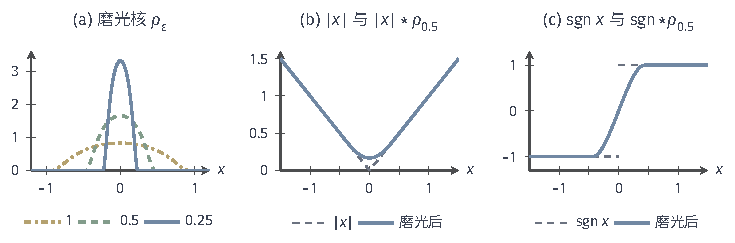
\includegraphics[width=124.4mm]{figures/02-abstract-mathematics/03-function-spaces/tikz/c4-mollifier/figure.pdf}
  \caption{一维磨光。(a)~磨光核$\rho_\varepsilon$，$\varepsilon=1,0.5,0.25$：支撑为$[-\varepsilon,\varepsilon]$，峰值约$0.829/\varepsilon$，面积均为$1$。(b)~$|x|$（虚线）与$|x|*\rho_{0.5}$（实线）：尖点被抹平，原点值约$0.167$，在$|x|\ge0.5$处两者重合。(c)~$\operatorname{sgn}x$与$\operatorname{sgn}*\rho_{0.5}$：后者光滑地从$-1$升到$1$，它恰好是(b)中光滑曲线的导数，体现$(|x|*\rho_\varepsilon)'=\operatorname{sgn}*\rho_\varepsilon$。}
  \label{fig:sob-mollifier}
\end{figure*}

\paragraph{$L^p$中的恢复}
要让磨光成为逼近，需要说明$u_\varepsilon\to u$。我们先考虑$\Omega=\mathbb R^d$且$u\in L^p(\mathbb R^d)$，$1\le p<\infty$；一般区域的情形随后用截断归结到这里。证明分三步。

第一步，磨光不放大$L^p$范数。$\rho_\varepsilon(x-\cdot)\,\mathrm dy$是质量为$1$的测度，对它使用Hölder不等式（$p>1$时把被积函数写成$|u|\rho_\varepsilon^{1/p}\cdot\rho_\varepsilon^{1/q}$），得
\[
 |u_\varepsilon(x)|^p\le\int|u(y)|^p\rho_\varepsilon(x-y)\,\mathrm dy .
\]
两边对$x$积分，非负被积函数可交换积分次序（定理~\ref{thm:analysis-tonelli-fubini}），而$\int\rho_\varepsilon(x-y)\,\mathrm dx=1$，于是
\begin{equation}
 \|u_\varepsilon\|_{L^p}\le\|u\|_{L^p} .
 \label{eq:sob-mollifier-contraction}
\end{equation}
同样的论证用于平均值之差，给出
\begin{equation}
 \|u_\varepsilon-u\|_{L^p}\le\sup_{|z|\le\varepsilon}\|u(\cdot-z)-u\|_{L^p} ,
 \label{eq:sob-mollifier-translation}
\end{equation}
因为$u_\varepsilon(x)-u(x)=\int[u(x-z)-u(x)]\rho_\varepsilon(z)\,\mathrm dz$也是关于质量为$1$的测度的平均。于是问题化为平移的连续性：小平移是否只引起小的$L^p$误差。

第二步，对紧支撑连续函数证明平移连续性。设$g$连续且支撑在紧集$K_0$内。由Heine--Cantor定理（定理~\ref{thm:metric-heine-cantor}），$g$一致连续，所以$\sup_x|g(x-z)-g(x)|\to0$（$z\to0$）。$|z|\le1$时差函数支撑在$\{x:\operatorname{dist}(x,K_0)\le1\}$内，这个集合的测度有限，记为$M$，于是$\|g(\cdot-z)-g\|_{L^p}\le M^{1/p}\sup_x|g(x-z)-g(x)|\to0$。

第三步，推广到一般$L^p$。由第~\ref{sec:fs-density-separability}节，紧支撑连续函数在$L^p(\mathbb R^d)$中稠密（$1\le p<\infty$）：先用简单函数逼近，再用连续截断逼近有限测度集合的示性函数。任给$\eta>0$，取这样的$g$使$\|u-g\|_{L^p}<\eta$。平移不改变$L^p$范数，所以
\[
 \begin{aligned}
 \|u(\cdot-z)-u\|_{L^p}&\le\|u(\cdot-z)-g(\cdot-z)\|_{L^p}+\|g(\cdot-z)-g\|_{L^p}+\|g-u\|_{L^p}\\
 &<2\eta+\|g(\cdot-z)-g\|_{L^p} .
 \end{aligned}
\]
令$z\to0$，右端的上极限不超过$2\eta$，而$\eta$任意，故平移连续性成立。代回式~\eqref{eq:sob-mollifier-translation}，得到$\|u_\varepsilon-u\|_{L^p}\to0$。

对一般开集$\Omega$和$u\in L^p(\Omega)$，取开集$V$，其闭包是$\Omega$内的紧集，记$\delta=\operatorname{dist}(V,\partial\Omega)$。把$u$在$\Omega$外补成零得到$\tilde u\in L^p(\mathbb R^d)$；当$\varepsilon<\delta$时，在$V$上$u_\varepsilon=\tilde u*\rho_\varepsilon$，所以$\|u_\varepsilon-u\|_{L^p(V)}\le\|\tilde u*\rho_\varepsilon-\tilde u\|_{L^p(\mathbb R^d)}\to0$。这就是磨光的局部$L^p$恢复。

$p=\infty$时结论不成立。在$(-1,1)$上，$H_\varepsilon=H*\rho_\varepsilon$连续，而$H$在原点两侧分别为$0$和$1$，所以在原点附近总有一侧满足$|H_\varepsilon-H|\ge1/2$，$\|H_\varepsilon-H\|_{L^\infty}$不趋于零。连续函数的一致极限仍连续，不连续的$L^\infty$函数不可能被连续函数一致逼近。

\paragraph{磨光与弱导数交换}
现在设$u$有弱导数$D^\alpha u\in L^1_{\mathrm{loc}}(\Omega)$。对$x\in\Omega_\varepsilon$，函数$y\mapsto\rho_\varepsilon(x-y)$是$\Omega$上的测试，其$y$导数满足$D_y^\alpha[\rho_\varepsilon(x-y)]=(-1)^{|\alpha|}(D^\alpha\rho_\varepsilon)(x-y)$。从式~\eqref{eq:sob-mollifier-derivative}出发，
\[
 D^\alpha u_\varepsilon(x)=(-1)^{|\alpha|}\int_\Omega u(y)\,D_y^\alpha[\rho_\varepsilon(x-y)]\,\mathrm dy
 =\int_\Omega D^\alpha u(y)\,\rho_\varepsilon(x-y)\,\mathrm dy ,
\]
第二个等号是弱导数的定义~\eqref{eq:sob-weak-derivative}用于这个测试。于是
\begin{equation}
 D^\alpha(u*\rho_\varepsilon)=(D^\alpha u)*\rho_\varepsilon\qquad\text{在 }\Omega_\varepsilon\text{ 上成立}.
 \label{eq:sob-mollifier-commute}
\end{equation}
左端是光滑函数的经典导数，右端是弱导数的磨光。图~\ref{fig:sob-mollifier}(b)(c)在$|x|$上验证了这一点：磨光后的$|x|$的经典导数，正是$\operatorname{sgn}x$的磨光。

把式~\eqref{eq:sob-mollifier-commute}与$L^p$恢复结合，就得到局部的光滑逼近。

\begin{theorem}[局部光滑逼近]
\label{thm:sob-local-approximation}
设$1\le p<\infty$，$u\in W^{k,p}(\Omega)$，$V$为开集且闭包是$\Omega$内的紧集。则$u_\varepsilon\in C^\infty(\Omega_\varepsilon)$，并且当$\varepsilon\to0$时$\|u_\varepsilon-u\|_{W^{k,p}(V)}\to0$。若$\Omega=\mathbb R^d$，则$\|u_\varepsilon-u\|_{W^{k,p}(\mathbb R^d)}\to0$。
\end{theorem}

\begin{proof}
光滑性已在前面证明。对每个$|\alpha|\le k$，由式~\eqref{eq:sob-mollifier-commute}，$D^\alpha u_\varepsilon-D^\alpha u=(D^\alpha u)_\varepsilon-D^\alpha u$在$V$上成立（$\varepsilon<\operatorname{dist}(V,\partial\Omega)$），而$D^\alpha u\in L^p(\Omega)$，由局部$L^p$恢复，它在$L^p(V)$中趋于零。有限多个分量都趋于零，Sobolev范数也趋于零。$\Omega=\mathbb R^d$时用全空间的恢复即可。
\end{proof}

这个定理是连接弱运算与经典计算的桥梁：凡是对光滑函数成立、又只涉及$W^{k,p}$范数连续量的等式或不等式，都可以先对$u_\varepsilon$证明，再令$\varepsilon\to0$。它对$W^{k,\infty}$不成立。例如任何$C^1$函数$v$在$(-1,1)$上都满足$\|v'-\operatorname{sgn}\|_{L^\infty}\ge1$：$v'$在原点连续，在原点附近的右侧与左侧分别接近同一个数$v'(0)$，而$\max(|v'(0)-1|,|v'(0)+1|)\ge1$。所以$|x|$不能在$W^{1,\infty}$范数下被$C^1$函数逼近。

\subsection{整域逼近与边界延拓}
\label{sec:sob-global-approximation}

定理~\ref{thm:sob-local-approximation}只在离边界有正距离的区域上逼近。靠近边界的地方，磨光半径必须越来越小，否则会读到区域外的值。解决办法是把函数切成许多块，每块离边界的距离不同，各自选择合适的磨光半径，再拼回去。切块需要一组光滑的权重。

\paragraph{局部有限的单位分解}
取递增的开集$G_j=\{x\in\Omega:|x|<j,\ \operatorname{dist}(x,\partial\Omega)>1/j\}$，$j\ge1$，并令$G_0=G_{-1}=\varnothing$。每个$G_j$的闭包是$\Omega$内的紧集，$\bigcup_jG_j=\Omega$。令
\[
 V_j=G_{j+1}\setminus\overline{G_{j-1}},\qquad j\ge1 .
\]
这些开集覆盖$\Omega$，并且是\term{局部有限}（locally finite）的：每个$x\in\Omega$属于某个$G_m$，而$G_m$只与$V_1,\ldots,V_{m+1}$相交，所以$x$的邻域$G_m$只与有限多个$V_j$相交。可以证明存在函数$\zeta_j\in C_c^\infty(V_j)$，满足$0\le\zeta_j\le1$，并且
\[
 \sum_{j\ge1}\zeta_j(x)=1\qquad(x\in\Omega).
\]
构造方法是：用引理~\ref{lem:sob-cutoff}在紧集$\overline{G_j}\setminus G_{j-1}$上取等于$1$、支撑在$V_j$内的截断$\eta_j$，则$\sum_i\eta_i$在每点是有限和且处处为正，令$\zeta_j=\eta_j/\sum_i\eta_i$。称$\{\zeta_j\}$为从属于覆盖$\{V_j\}$的\term{单位分解}（partition of unity）。

图~\ref{fig:sob-partition-unity}在$\Omega=(0,1)$上画出了一组这样的权重，那里用到边界距离的对数作分层，与上面的$G_j$略有不同，但性质相同：每个权重的支撑紧含于区域，越靠近边界的权重支撑越窄，每一点只有有限个（图中至多两个）权重非零，总和恒为$1$。

\begin{figure}[!htb]
  \centering
  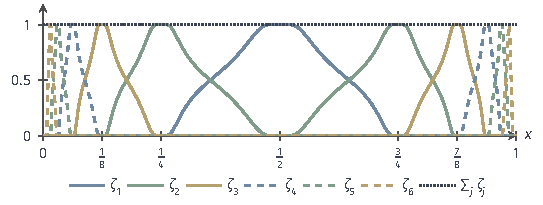
\includegraphics[width=92.0mm]{figures/02-abstract-mathematics/03-function-spaces/tikz/c4-partition-unity/figure.pdf}
  \caption{$\Omega=(0,1)$上的局部有限单位分解。记$s=\min(x,1-x)$为到边界的距离，$\zeta_j$支撑在$2^{-j-1}\le s\le2^{-j+1}$内，紧含于$(0,1)$；图中画出$\zeta_1,\ldots,\zeta_6$，每点至多两个权重非零，所有权重之和恒为$1$（点线）。越靠近边界，权重越密集，对应的磨光半径也要越小。}
  \label{fig:sob-partition-unity}
\end{figure}

\begin{theorem}[整域光滑逼近]
\label{thm:sob-meyers-serrin}
设$\Omega\subset\mathbb R^d$为任意开集，$k\ge0$，$1\le p<\infty$。则$C^\infty(\Omega)\cap W^{k,p}(\Omega)$在$W^{k,p}(\Omega)$中稠密。
\end{theorem}

\begin{proof}
固定$u\in W^{k,p}(\Omega)$与$\eta>0$。

第一步，分块。令$u_j=\zeta_ju$。由第~\ref{sec:sob-weak-derivative-def}节与光滑函数相乘的乘积法则（对高阶导数反复使用），$u_j\in W^{k,p}(\Omega)$，其各阶弱导数是$\zeta_j$的导数与$u$的弱导数的乘积之和，支撑在$V_j$内。由于$\zeta_j$紧支撑在$\Omega$内，把$u_j$在$\Omega$外补成零后属于$W^{k,p}(\mathbb R^d)$：对$\mathbb R^d$上的测试$\varphi$，用一个在$\operatorname{supp}\zeta_j$上为$1$、支撑在$\Omega$内的截断$\chi$，有$\int u_jD^\alpha\varphi=\int u_jD^\alpha(\chi\varphi)$，而$\chi\varphi$是$\Omega$上的测试。

第二步，逐块磨光并分配误差。对每个$j$，由定理~\ref{thm:sob-local-approximation}在$\mathbb R^d$上的结论，取$\varepsilon_j>0$足够小，使$v_j=u_j*\rho_{\varepsilon_j}$满足
\[
 \|v_j-u_j\|_{W^{k,p}(\mathbb R^d)}<\eta\,2^{-j},
\]
并且$\operatorname{supp}v_j\subset W_j:=G_{j+2}\setminus\overline{G_{j-2}}$。后一要求可以满足：$v_j$的支撑落在$\operatorname{supp}u_j$的$\varepsilon_j$邻域内，而$\overline{G_{j+1}}\subset G_{j+2}$、$\overline{G_{j-2}}\subset G_{j-1}$都是紧集含于开集，$V_j$与$W_j$的补集之间有正的间隔，取$\varepsilon_j$小于这个间隔即可。这里给第$j$块分配误差$\eta2^{-j}$，是为了让总和不超过$\eta$。

第三步，拼合。令$v=\sum_jv_j$。每点有邻域只与有限多个$W_j$相交，所以在这个邻域上$v$是有限个光滑函数之和，$v\in C^\infty(\Omega)$。同理$u=\sum_ju_j$在每个$G_m$上也只是有限和。于是在$G_m$上
\[
 \|v-u\|_{W^{k,p}(G_m)}\le\sum_j\|v_j-u_j\|_{W^{k,p}(\mathbb R^d)}<\sum_j\eta2^{-j}=\eta .
\]
令$m\to\infty$，由单调收敛定理（第~\ref{sec:measure-general-structure}节），$\|v-u\|_{W^{k,p}(\Omega)}\le\eta$。特别地$v\in W^{k,p}(\Omega)$。
\end{proof}

这个定理对任意开集成立，连边界的形状都不需要。但要读清它给出的是什么：逼近函数在$\Omega$\emph{内部}光滑，可能在边界附近剧烈振荡，并不是“光滑到边界”的函数，更不是紧支撑在$\Omega$内的测试函数。$C_c^\infty(\Omega)$在$W^{k,p}(\Omega)$中一般\emph{不}稠密。以$(0,1)$上的常数$1$为例：每个$\varphi\in C_c^\infty(0,1)$在端点附近为零，由式~\eqref{eq:sob-1d-sup-bound}（$p=2$，$L=1$），
\[
 1=|1-\varphi(0)|\le\|1-\varphi\|_{L^2}+\|(1-\varphi)'\|_{L^2}\le\sqrt2\,\|1-\varphi\|_{H^1},
\]
所以常数$1$到$C_c^\infty(0,1)$的$H^1$距离至少是$1/\sqrt2$。测试函数的闭包把“边界值为零”的信息保留了下来，这将在第~\ref{sec:sob-poincare}节定义$H_0^1$。

\paragraph{光滑到边界：从半空间反射开始}
许多论证需要更强的逼近：逼近函数在闭区域$\overline\Omega$上光滑，即是某个$C_c^\infty(\mathbb R^d)$函数在$\Omega$上的限制。思路是先把$u$延拓成全空间上的Sobolev函数，再在全空间磨光，最后限制回$\Omega$。延拓是关键，而延拓方式的好坏取决于边界。

最简单的区域是半空间$\mathbb R^d_+=\{x=(x',x_d):x_d>0\}$，这里$x'\in\mathbb R^{d-1}$。对光滑到边界的$u$，作偶反射
\[
 Eu(x',x_d)=u(x',|x_d|).
\]
它在$x_d=0$处连续，但沿$x_d$方向一般出现尖点。像$|x|$那样在两侧分别分部积分，边界面上的项因两侧的值相同而相消，所以$Eu$有弱导数：对$j<d$，$\partial_jEu(x',x_d)=(\partial_ju)(x',|x_d|)$；对$j=d$，$\partial_dEu(x',x_d)=\operatorname{sgn}(x_d)\,(\partial_du)(x',|x_d|)$。两侧对称，所以
\[
 \|Eu\|_{W^{1,p}(\mathbb R^d)}^p=2\,\|u\|_{W^{1,p}(\mathbb R^d_+)}^p .
\]
一般的$u\in W^{1,p}(\mathbb R^d_+)$可以先向区域内部平移一小段再磨光，得到光滑到边界的逼近，再由上式把延拓推广过去；这一细节属于补充，这里不展开。

与偶反射对照，零延拓（在$x_d<0$处令$u=0$）通常不行：若$u$在边界面上的值不为零，零延拓在边界面上产生跳跃，按阶跃函数的计算，它的$x_d$方向广义导数含有一个集中在边界面上的项，不是局部可积函数。图~\ref{fig:sob-reflection}在一维比较了两种延拓。只有当$u$的边界值为零时（确切含义见第~\ref{sec:sob-trace}节），零延拓才保持在$W^{1,p}$中。高阶空间中偶反射也不够，因为$x_d$方向的导数在反射后改变符号而跳跃；可以改用$Eu(x',x_d)=-3u(x',-x_d)+4u(x',-x_d/2)$（$x_d<0$），容易核对它在边界面上与$u$的值和一阶法向导数都相接。

\begin{figure}[!htb]
  \centering
  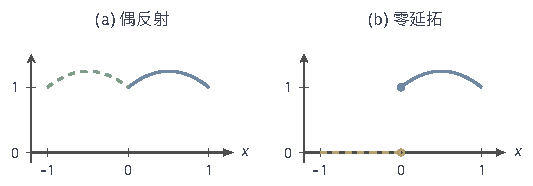
\includegraphics[width=90.2mm]{figures/02-abstract-mathematics/03-function-spaces/tikz/c4-reflection/figure.pdf}
  \caption{半区间上的两种延拓，$u(x)=1+x-x^2$（$0\le x\le1$），$u(0)=1$。(a)~偶反射$Eu(x)=u(|x|)$（虚线为延拓部分）：在原点连续而有尖点，弱导数$\operatorname{sgn}(x)u'(|x|)$局部可积，延拓保持在$W^{1,p}$中。(b)~零延拓：在原点跳跃$u(0)=1$，广义导数含$\delta_0$项，延拓不在$W^{1,p}$中。}
  \label{fig:sob-reflection}
\end{figure}

\paragraph{Lipschitz区域与延拓}
一般区域的边界可以弯曲，但只要它在局部可以拉直成半空间，就能沿用反射。

\begin{definition}[Lipschitz区域]
\label{def:sob-lipschitz-domain}
称有界开集$\Omega\subset\mathbb R^d$为\term{Lipschitz区域}（Lipschitz domain），若对每个$x_0\in\partial\Omega$，存在$r>0$、一个以$x_0$为原点的旋转后的坐标系$(x',x_d)$和Lipschitz函数$\gamma:\mathbb R^{d-1}\to\mathbb R$，使
\[
 \Omega\cap B(x_0,r)=\{x\in B(x_0,r):x_d>\gamma(x')\}.
\]
\end{definition}

也就是说，在每个边界点附近，区域位于一个Lipschitz函数图像的上方，边界就是这个图像。球、立方体、凸多面体都是Lipschitz区域：立方体的棱角处边界不光滑，但仍是局部的Lipschitz图像。挖去一条线段的圆盘（割缝圆盘）不是：割缝两侧都是区域，区域不能只位于割缝的一侧。尖角向内收缩得比任何Lipschitz图像都快的区域也不是。

\begin{theorem}[Lipschitz区域上的延拓]
\label{thm:sob-extension}
设$\Omega$为有界Lipschitz区域，$1\le p<\infty$。存在有界线性算子$E:W^{1,p}(\Omega)\to W^{1,p}(\mathbb R^d)$，使$Eu=u$在$\Omega$上几乎处处成立，并且所有$Eu$都支撑在同一个有界集合内。
\end{theorem}

证明思路如下，细节属于补充阅读。边界是紧集，可以用有限个满足定义的球$B(x_i,r_i)$覆盖，再加上一个紧含于$\Omega$的开集覆盖内部；取从属于这有限个开集的单位分解，把$u$分成有限块。内部那块直接零延拓，它在边界附近本来就是零。每个边界块用变换$(x',x_d)\mapsto(x',x_d-\gamma(x'))$拉直：这个变换和它的逆都是Lipschitz的，可以证明它们把$W^{1,p}$函数变成$W^{1,p}$函数，范数只差一个由$\gamma$的Lipschitz常数决定的倍数。拉直后在半空间上作偶反射，再变换回去。有限多块的延拓相加，得到$Eu$。这里每一步都需要边界是局部的Lipschitz图像，割缝圆盘之所以失败，正是因为割缝两侧都有区域，无法只向一侧反射。

\begin{theorem}[光滑到边界的逼近]
\label{thm:sob-smooth-up-to-boundary}
设$\Omega$为有界Lipschitz区域，$1\le p<\infty$。则$C_c^\infty(\mathbb R^d)$中函数在$\Omega$上的限制在$W^{1,p}(\Omega)$中稠密。
\end{theorem}

\begin{proof}
对$u\in W^{1,p}(\Omega)$，由定理~\ref{thm:sob-extension}得到紧支撑的$Eu\in W^{1,p}(\mathbb R^d)$。由定理~\ref{thm:sob-local-approximation}，$Eu*\rho_\varepsilon\to Eu$在$W^{1,p}(\mathbb R^d)$中成立，而$Eu*\rho_\varepsilon\in C_c^\infty(\mathbb R^d)$。限制到$\Omega$上，范数只会变小，所以$\|(Eu*\rho_\varepsilon)|_\Omega-u\|_{W^{1,p}(\Omega)}\le\|Eu*\rho_\varepsilon-Eu\|_{W^{1,p}(\mathbb R^d)}\to0$。
\end{proof}

记这类限制函数的全体为$C^\infty(\overline\Omega)$。与定理~\ref{thm:sob-meyers-serrin}比较，它多了边界正则性的条件，换来了在闭区域上光滑、各阶导数连续到边界的逼近函数。下一节的边界迹就要用到这一点：对光滑到边界的函数，边界值有经典含义，再用逼近推广到整个Sobolev空间。

% 第4章第5节：正则性、紧性与边界（嵌入与连续代表、紧嵌入、边界迹、零边界与Poincaré不等式）。

\section{正则性、紧性与边界}
\label{sec:sob-regularity}

Sobolev空间完备，光滑函数在其中稠密，但第~\ref{sec:sob-completeness}节末尾留下的问题还没有回答。本节分别研究四个问题：导数的积分控制能把函数值控制到什么程度；范数有界的函数列能否抽出强收敛子列；体积上的函数怎样拥有边界值；去掉常数方向以后，能否只用导数控制函数本身。四个问题都靠导数控制，但各自需要的条件不同，得到的结论也不能互相替代。

本节除特别说明外，都在有界Lipschitz区域$\Omega\subset\mathbb R^d$上讨论，并且只处理一阶空间$W^{1,p}(\Omega)$。区域有界保证小指数的$L^q$范数受大指数控制（$\|u\|_{L^q}\le|\Omega|^{1/q-1/p}\|u\|_{L^p}$，$q\le p$），边界为Lipschitz保证第~\ref{sec:sob-global-approximation}节的延拓与光滑到边界的逼近可用。

\subsection{积分指数与连续代表}
\label{sec:sob-embedding}

一维时，第~\ref{sec:sob-absolute-continuity}节证明了$W^{1,p}(a,b)$的元素都有连续代表，$p>1$时还是Hölder连续的。可是式~\eqref{eq:sob-power-membership}给出$|x|^{-1/4}\in W^{1,2}(B)$（$B$为$\mathbb R^3$中的单位球），它在原点无界。可见在高维，导数平方可积不足以保证连续。究竟是什么决定了结论？

\paragraph{缩放解释}
设想对全空间上的光滑紧支撑函数$u$有不等式$\|u\|_{L^q(\mathbb R^d)}\le C\|\nabla u\|_{L^p(\mathbb R^d)}$，常数$C$不依赖$u$。把$u$换成$u_\lambda(x)=u(\lambda x)$，$\lambda>0$。由换元$y=\lambda x$，
\[
 \|u_\lambda\|_{L^q}=\lambda^{-d/q}\|u\|_{L^q},\qquad\|\nabla u_\lambda\|_{L^p}=\lambda^{1-d/p}\|\nabla u\|_{L^p} .
\]
不等式对所有$\lambda$成立，两边的$\lambda$指数必须相等，否则令$\lambda\to0$或$\lambda\to\infty$就会破坏它。于是$-d/q=1-d/p$，即
\begin{equation}
 \frac1q=\frac1p-\frac1d,\qquad q=p^*:=\frac{dp}{d-p}\quad(1\le p<d).
 \label{eq:sob-sobolev-exponent}
\end{equation}
称$p^*$为$p$的\term{Sobolev共轭指数}（Sobolev conjugate exponent）。缩放论证只说明了指数必须是什么，并没有证明不等式成立；但它揭示了维数的作用：在$d$维中，把函数压缩到小尺度，导数的$L^p$范数按$\lambda^{1-d/p}$变化，$d$越大、$p$越小，导数就越“看不见”尖锐的集中。当$p>d$时，同样的计算用于Hölder商$|u(x)-u(y)|/|x-y|^\gamma$，它按$\lambda^\gamma$缩放，与$\lambda^{1-d/p}$匹配要求$\gamma=1-d/p$。

\begin{theorem}[Sobolev嵌入]
\label{thm:sob-embedding}
设$\Omega\subset\mathbb R^d$为有界Lipschitz区域。
\begin{enumerate}
 \item 若$1\le p<d$，则$W^{1,p}(\Omega)\subset L^{p^*}(\Omega)$，并存在常数$C$使$\|u\|_{L^{p^*}}\le C\|u\|_{W^{1,p}}$。由区域有界，对$1\le q\le p^*$也有$\|u\|_{L^q}\le C_q\|u\|_{W^{1,p}}$。
 \item 若$d<p<\infty$，则每个$u\in W^{1,p}(\Omega)$有一个在$\overline\Omega$上$\gamma=1-d/p$阶Hölder连续的代表$\tilde u$，并且
 \[
  \sup_{\overline\Omega}|\tilde u|+\sup_{x\neq y}\frac{|\tilde u(x)-\tilde u(y)|}{|x-y|^{\gamma}}\le C\|u\|_{W^{1,p}} .
 \]
\end{enumerate}
\end{theorem}

一个包含关系连同范数控制，称为\term{连续嵌入}（continuous embedding）：包含映射是有界线性算子。图~\ref{fig:sob-embedding-exponents}(a)在$(p,d)$平面上标出两种情形，(b)画出$p^*$随$p$的变化。$H^1=W^{1,2}$在$d=1$时落在Hölder一侧，得到$C^{0,1/2}$，与式~\eqref{eq:sob-1d-holder}一致；$d=3$时落在另一侧，$2^*=6$，得到$L^6$；$d=2$恰好在分界线上。

\begin{figure}[!htb]
  \centering
  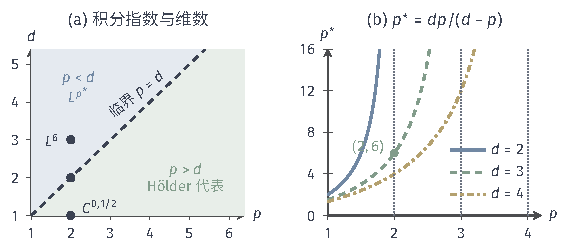
\includegraphics[width=96.3mm]{figures/02-abstract-mathematics/03-function-spaces/tikz/c4-embedding-exponents/figure.pdf}
  \caption{$W^{1,p}$的嵌入由积分指数与维数共同决定。(a)~$(p,d)$平面：$p<d$（蓝）时嵌入$L^{p^*}$，$p>d$（绿）时有Hölder连续代表，虚线$p=d$为临界情形；三个点是$p=2$、$d=1,2,3$，分别得到$C^{0,1/2}$、临界与$L^6$。(b)~$p^*=dp/(d-p)$随$p$增大而增大，$p\to d$时趋于无穷；$d=3$、$p=2$时$p^*=6$。}
  \label{fig:sob-embedding-exponents}
\end{figure}

\paragraph{幂函数检验指数的精确性}
回到$B\subset\mathbb R^d$上的$u=|x|^{-a}$。由式~\eqref{eq:sob-power-membership}，$u\in W^{1,p}(B)$当且仅当$(a+1)p<d$，即$a<d/p-1$；而$u\in L^q(B)$当且仅当$aq<d$。取$q=p^*$，条件$ap^*<d$化为$a<d/p^*=d/p-1$，与前者完全相同。所以每个在$W^{1,p}(B)$中的幂函数都在$L^{p^*}(B)$中，而对任何$q>p^*$，取$a$略小于$d/p-1$，便得到$W^{1,p}(B)$中不属于$L^q(B)$的函数：$p^*$不能再提高。$d=3$、$p=2$时，$a<1/2$的幂函数都在$L^6$中，且无界，这说明$p<d$时一般没有连续代表。

\paragraph{两种结论的机制}
两种情形的证明都从光滑函数出发，再借定理~\ref{thm:sob-smooth-up-to-boundary}推广。$p<d$的情形，先对$\mathbb R^d$上的光滑紧支撑函数证明$\|u\|_{L^{d/(d-1)}}\le\|\nabla u\|_{L^1}$：沿每个坐标方向，$|u(x)|\le\int_{\mathbb R}|\partial_ju|\,\mathrm dx_j$，把$d$个这样的估计相乘开$d-1$次根，再逐个坐标积分并反复使用Hölder不等式。一般的$p$由对$|u|^s$（适当的$s>1$）使用这一估计得到；有界Lipschitz区域上再用延拓算子转移到全空间。这一证明较长，属于补充阅读。

$p>d$的情形可以看出Hölder指数从哪里来。对光滑函数和以$x$为中心、半径$r$的球$B_r$，把$u(x)-u(y)$写成沿线段的导数积分，再对$y\in B_r$取平均，可以得到
\[
 \Bigl|u(x)-\frac{1}{|B_r|}\int_{B_r}u\,\mathrm dy\Bigr|\le C\int_{B_r}\frac{|\nabla u(y)|}{|x-y|^{d-1}}\,\mathrm dy .
\]
右端用Hölder不等式拆成$\|\nabla u\|_{L^p}$与$\bigl(\int_{B_r}|x-y|^{-(d-1)q}\mathrm dy\bigr)^{1/q}$，$q$为共轭指数。后一积分有限当且仅当$(d-1)q<d$，即$p>d$，此时它等于常数乘$r^{1-d/p}$。于是函数值与它在半径$r$的球上的平均之差不超过$Cr^{1-d/p}\|\nabla u\|_{L^p}$；两个相距$r$的点都和同一个球的平均比较，就得到$\gamma=1-d/p$阶的Hölder估计。$p\le d$时核$|x-y|^{1-d}$的$q$次幂不可积，这一步失效。两种结论的区别正在这里：$p<d$时得到的是更高的可积性，由体积上的积分累计；$p>d$时得到的是逐点的振荡控制，靠的是局部平均与中心值的比较。更高的可积性不等于连续，$L^{p^*}$中的函数仍可以无界。

\paragraph{临界情形$p=d$}
$d\ge2$、$p=d$时，两种结论都差一点。一方面，对每个有限的$q$，$W^{1,d}(\Omega)\subset L^q(\Omega)$：区域有界时$W^{1,d}(\Omega)\subset W^{1,s}(\Omega)$对每个$s<d$成立，而$s\to d$时$s^*=ds/(d-s)\to\infty$，所以任意有限$q$都被某个$s^*$超过。另一方面，$W^{1,d}$中的函数一般无界。在单位球$B\subset\mathbb R^d$中取
\[
 u(x)=\ln\ln\frac{e}{|x|} .
\]
记$r=|x|$，$s=\ln(e/r)\ge1$，则$|\nabla u|=1/(rs)$。按球坐标，$\int_B|\nabla u|^d\,\mathrm dx$与$\int_0^1\frac{r^{d-1}}{r^ds^d}\,\mathrm dr=\int_0^1\frac{\mathrm dr}{r\,(\ln(e/r))^d}$成正比，换元$s=\ln(e/r)$后化为$\int_1^\infty s^{-d}\,\mathrm ds$，$d\ge2$时有限；$u$本身只以$\ln\ln$的速度增长，属于$L^d(B)$。所以$u\in W^{1,d}(B)$，却在原点趋于无穷。

一维的$p=1=d$不受这一否定结论影响：第~\ref{sec:sob-absolute-continuity}节已经证明$W^{1,1}(a,b)$的元素有绝对连续代表，当然有界。原因是一维时单点的“容量”不为零：从$x$到$y$只有一条路径，函数的变化必须全部经过它，而在高维中，函数可以绕开一个点集中增长。

\paragraph{高阶空间}
同样的指数比较可以推广到$W^{k,p}$：每多一阶导数，在缩放中多出一个因子$\lambda$。若$kp<d$，则$W^{k,p}(\Omega)\subset L^q(\Omega)$，$1/q=1/p-k/d$；若$kp>d$，则函数有连续代表。特别地，$H^k(\Omega)$的元素在$k>d/2$时有连续代表，并且$\sup|\tilde u|\le C\|u\|_{H^k}$。这一结论使每个点值读取$u\mapsto\tilde u(x)$都是$H^k$上的有界线性泛函，第~\ref{chap:rkhs}章将以此为例说明哪些Hilbert函数空间具有连续的点值。分数阶空间与临界情形的完整分类这里不展开。

\subsection{有界函数列的紧性}
\label{sec:sob-compactness}

第~\ref{sec:sob-completeness}节的例子$u_n=\sin(n\pi x)/(n\pi)$在$H^1(0,1)$中有界，不在$H^1$中收敛，却在$L^2$中收敛。这不是巧合：导数的统一控制阻止了函数在小尺度上剧烈振荡，从而在较弱的范数下迫使序列聚集。

\begin{theorem}[紧嵌入]
\label{thm:sob-rellich}
设$\Omega\subset\mathbb R^d$为有界Lipschitz区域，$1\le p<\infty$。则$W^{1,p}(\Omega)$中的每个有界序列都有一个在$L^p(\Omega)$中收敛的子列。更一般地，$1\le p<d$时可以把$L^p$换成$L^q$，$1\le q<p^*$；$p\ge d$时可以换成任意有限$q$的$L^q$。
\end{theorem}

称这样的包含为\term{紧嵌入}（compact embedding）：包含映射把有界集映成相对紧集，按第~\ref{sec:ose-compact-def}节的说法，它是紧算子。下面给出$L^p$情形的证明，其中用到的延拓定理只给出了证明思路；$L^q$情形的推广由插值不等式得到，从略。

\begin{proof}
设$\|u_n\|_{W^{1,p}(\Omega)}\le M$。只需证明集合$\mathcal F=\{u_n\}$在$L^p(\Omega)$中全有界（第~\ref{sec:metric-totally-bounded}节）：$L^p$完备，完备空间中全有界集的闭包是紧的（定理~\ref{thm:metric-compact-complete-tb}），紧集中的序列有收敛子列。

第一步，转移到全空间。用定理~\ref{thm:sob-extension}的延拓算子，令$w_n=Eu_n$，则$\|w_n\|_{W^{1,p}(\mathbb R^d)}\le\|E\|M=:M'$，且所有$w_n$支撑在同一个有界集合内。只需证明$\{w_n\}$在$L^p(\mathbb R^d)$中全有界，限制到$\Omega$上不增大距离。

第二步，统一的平移估计。对光滑紧支撑函数$w$，$w(x+z)-w(x)=\int_0^1\nabla w(x+tz)\cdot z\,\mathrm dt$，两边取$L^p$范数并把范数移进对$t$的积分（Minkowski积分不等式），得
\[
 \|w(\cdot+z)-w\|_{L^p}\le|z|\,\|\nabla w\|_{L^p} .
\]
两边对$W^{1,p}$范数连续，由定理~\ref{thm:sob-local-approximation}的逼近，它对每个$w\in W^{1,p}(\mathbb R^d)$成立。结合式~\eqref{eq:sob-mollifier-translation}，
\[
 \|w_n*\rho_\varepsilon-w_n\|_{L^p}\le\varepsilon M'\qquad\text{对所有 }n\text{ 一致成立}.
\]
这一步是关键：导数的统一界把所有函数的磨光误差统一控制住了。

第三步，固定$\varepsilon$后的有限网。固定$\varepsilon$，函数$w_n*\rho_\varepsilon$都支撑在同一个紧集$K$内，并且由Hölder不等式，
\[
 |w_n*\rho_\varepsilon(x)|\le\|\rho_\varepsilon\|_{L^q}M',\qquad|\nabla(w_n*\rho_\varepsilon)(x)|\le\|\nabla\rho_\varepsilon\|_{L^q}M' ,
\]
$q$为共轭指数。所以这族函数在$K$上一致有界并有统一的Lipschitz常数。在$K$上取一个间距为$h$的有限网格，每个函数由它在网格点上的值确定到$\|\nabla\rho_\varepsilon\|_{L^q}M'\sqrt d\,h$以内；网格点上的值落在一个有界区间内，把这个区间分成有限多段，就把整族函数分成有限多组，每组内函数的一致距离任意小。一致距离乘$|K|^{1/p}$控制$L^p$距离，所以$\{w_n*\rho_\varepsilon\}$在$L^p$中全有界。这一论证正是第~\ref{sec:apx-arzela-ascoli}节Arzelà--Ascoli定理的机制。

第四步，合并。任给$\eta>0$，先取$\varepsilon$使$\varepsilon M'<\eta/3$，再取$\{w_n*\rho_\varepsilon\}$的有限$\eta/3$网$\{g_1,\ldots,g_N\}$。对每个$n$，选$g_i$与$w_n*\rho_\varepsilon$相距小于$\eta/3$，则$\|w_n-g_i\|_{L^p}<\varepsilon M'+\eta/3<\eta$。所以$\{w_n\}$有有限$\eta$网，全有界。
\end{proof}

证明清楚地显示了三种条件各自的职责。导数的统一界给出统一的平移估计，使磨光误差与$n$无关；区域有界（经延拓后支撑在同一有界集内）使固定尺度的函数族只需有限个网格点描述；目标范数$L^p$比$W^{1,p}$弱，才允许用磨光后的函数近似原函数。

\paragraph{与弱收敛子列的对照}
$1<p<\infty$时，$W^{1,p}(\Omega)$是自反空间，由第~\ref{sec:lfo-weak-subsequence}节，有界序列有弱收敛子列$u_{n_k}\rightharpoonup u$。紧嵌入把这一结论加强了：同一子列在$L^p$中\emph{强}收敛到$u$。原因是紧算子把弱收敛序列映成强收敛序列。在优化与变分问题中，这一组合经常这样使用：从极小化序列的有界性抽出弱收敛子列，再借紧嵌入让低阶项强收敛。但紧嵌入本身只是关于函数列的结论，并不是某个具体方程的可解性定理；把它用于具体问题时，还需要说明目标函数或方程项怎样在这种收敛下保持。

\paragraph{临界指数处的失紧}
定理~\ref{thm:sob-rellich}中$q<p^*$是严格不等式。在临界指数$q=p^*$处，嵌入仍连续，但不再是紧的。取$\varphi\in C_c^\infty(B)$非零，$B$为单位球，$1\le p<d$，令
\[
 u_\lambda(x)=\lambda^{(d-p)/p}\varphi(\lambda x),\qquad\lambda\ge1 .
\]
$u_\lambda$支撑在半径$1/\lambda$的球内。由缩放公式，$\|\nabla u_\lambda\|_{L^p}=\|\nabla\varphi\|_{L^p}$与$\|u_\lambda\|_{L^{p^*}}=\|\varphi\|_{L^{p^*}}$都不随$\lambda$改变，而$\|u_\lambda\|_{L^p}=\lambda^{-1}\|\varphi\|_{L^p}\to0$。所以$(u_\lambda)$在$W^{1,p}(B)$中有界。若某个子列在$L^{p^*}(B)$中收敛，由于它在$L^p$中收敛到$0$，$L^{p^*}$极限也只能是$0$（$L^{p^*}$收敛推出$L^p$收敛），与$\|u_\lambda\|_{L^{p^*}}$恒为常数矛盾。函数的质量向一点集中，在$L^{p^*}$中“看起来”一直一样大，却不收敛到任何东西。图~\ref{fig:sob-compactness-loss}(a)画出$d=3$、$p=2$时的径向剖面$u_\lambda(r)=\lambda^{1/2}\psi(\lambda r)$。

\begin{figure}[!htb]
  \centering
  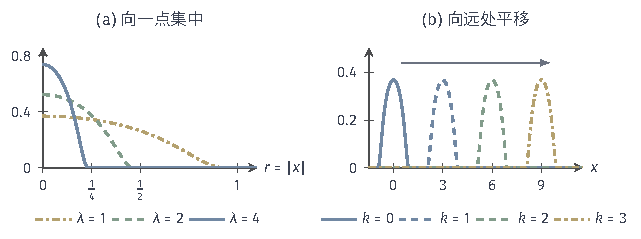
\includegraphics[width=108.6mm]{figures/02-abstract-mathematics/03-function-spaces/tikz/c4-compactness-loss/figure.pdf}
  \caption{两种失去紧性的方式。(a)~临界集中：$d=3$、$p=2$，$u_\lambda(x)=\lambda^{1/2}\psi(\lambda|x|)$的径向剖面，$\lambda=1,2,4$；峰值按$\lambda^{1/2}$升高，支撑半径按$1/\lambda$缩小，$\|\nabla u_\lambda\|_{L^2}$与$\|u_\lambda\|_{L^6}$不变，$\|u_\lambda\|_{L^2}\to0$。(b)~无界区域上的平移：$\psi(x-3k)$，$k=0,1,2,3$，形状和范数都不变，支撑互不相交，向远处逃逸。}
  \label{fig:sob-compactness-loss}
\end{figure}

\paragraph{无界区域上的逃逸}
区域有界的条件也不能去掉。在$\mathbb R^d$上取非零$\varphi\in C_c^\infty(\mathbb R^d)$与单位向量$e$，令$u_n(x)=\varphi(x-3n\,r_0e)$，其中$r_0$使$\operatorname{supp}\varphi\subset B(0,r_0)$。每个$u_n$的$W^{1,p}$范数都等于$\varphi$的范数，支撑两两不交，所以$\|u_n-u_m\|_{L^p}=2^{1/p}\|\varphi\|_{L^p}$（$n\neq m$），任何子列都不是$L^p$中的Cauchy列。函数没有集中，而是整体跑到了无穷远（图~\ref{fig:sob-compactness-loss}(b)，一维时取$\varphi=\psi$、$r_0=1$）。有界区域上，延拓后支撑被限制在同一有界集内，这种逃逸不会发生。

\subsection{边界迹}
\label{sec:sob-trace}

许多问题要给函数指定边界值。可是$W^{1,p}(\Omega)$的元素是几乎处处等价类，而$\partial\Omega$在$\mathbb R^d$中是Lebesgue零测集，任意修改一个代表在边界上的值，得到的仍是同一个元素。“$u$在边界上的值”因此需要重新定义，而不能取一个代表直接限制。

\paragraph{一维端点估计}
一维的答案已经有了。$u\in H^1(a,b)$有唯一的连续代表，式~\eqref{eq:sob-1d-sup-bound}在端点给出
\[
 |\tilde u(a)|\le L^{-1/2}\|u\|_{L^2}+L^{1/2}\|u'\|_{L^2}\le C\|u\|_{H^1(a,b)} .
\]
端点值由$H^1$范数控制，这正是高维要推广的东西。只有$L^2$控制是不够的：$u_n(x)=\max(1-nx,0)$在$(0,1)$上满足$u_n(0)=1$，而$\|u_n\|_{L^2}^2=\int_0^{1/n}(1-nx)^2\,\mathrm dx=1/(3n)\to0$，端点值不受$L^2$范数控制。

\paragraph{半空间上的迹估计}
高维的关键估计可以在半空间上完整证明。设$u\in C_c^\infty(\mathbb R^d)$，限制在$\overline{\mathbb R^d_+}$上考虑。固定$x'\in\mathbb R^{d-1}$，沿$x_d$方向从边界点$(x',0)$向内积分（图~\ref{fig:sob-trace}(b)）：$|u(x',t)|^2$在$t$大时为零，所以
\[
 \begin{aligned}
 |u(x',0)|^2&=-\int_0^\infty\partial_t\bigl(|u(x',t)|^2\bigr)\,\mathrm dt\\
 &\le2\int_0^\infty|u|\,|\partial_du|\,\mathrm dt\le\int_0^\infty\bigl(|u|^2+|\partial_du|^2\bigr)\,\mathrm dt ,
 \end{aligned}
\]
最后一步用了$2ab\le a^2+b^2$。再对$x'\in\mathbb R^{d-1}$积分，得到
\begin{equation}
 \int_{\mathbb R^{d-1}}|u(x',0)|^2\,\mathrm dx'\le\|u\|_{L^2(\mathbb R^d_+)}^2+\|\partial_du\|_{L^2(\mathbb R^d_+)}^2\le\|u\|_{H^1(\mathbb R^d_+)}^2 .
 \label{eq:sob-half-space-trace}
\end{equation}
边界值的$L^2$大小被体积上函数和法向导数的$L^2$大小控制。这与一维端点估计是同一个机制：沿着垂直于边界的每一条线，都是一个一维问题。

\begin{figure}[!htb]
  \centering
  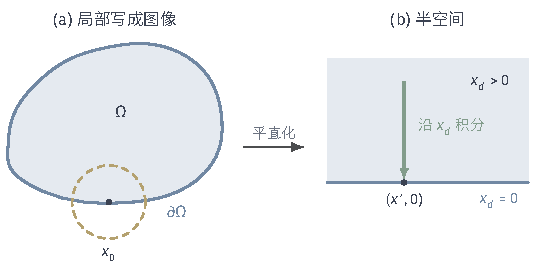
\includegraphics[width=90.3mm]{figures/02-abstract-mathematics/03-function-spaces/tikz/c4-trace/figure.pdf}
  \caption{边界迹的局部化与平直化。(a)~有界Lipschitz区域$\Omega$：边界点$x_0$附近的球（虚线）内，边界是Lipschitz函数的图像，区域位于图像一侧。(b)~拉直后成为半空间$\{x_d>0\}$：从边界点$(x',0)$沿$x_d$方向向内积分，边界值的平方被这条线上$|u|^2+|\partial_du|^2$的积分控制，再对$x'$积分即得式~\eqref{eq:sob-half-space-trace}。}
  \label{fig:sob-trace}
\end{figure}

\paragraph{Lipschitz区域上的迹定理}
在一般的有界Lipschitz区域上，边界需要配上\term{表面测度}（surface measure）$\mathrm dS$。在定义~\ref{def:sob-lipschitz-domain}的一个局部图像$x_d=\gamma(x')$上，约定$\mathrm dS=\sqrt{1+|\nabla\gamma(x')|^2}\,\mathrm dx'$；Lipschitz函数几乎处处可微且梯度有界，所以这个因子在$1$与$\sqrt{1+\mathrm{Lip}(\gamma)^2}$之间，边界上的$L^2$范数与拉直后$\mathbb R^{d-1}$上的$L^2$范数相差有界倍数。不同局部图像重叠处给出相同的测度，这里不加证明地使用这一点。记$L^2(\partial\Omega)=L^2(\partial\Omega,\mathrm dS)$。

\begin{theorem}[迹定理]
\label{thm:sob-trace}
设$\Omega$为有界Lipschitz区域。存在常数$C$，使所有$u\in C^\infty(\overline\Omega)$满足
\begin{equation}
 \|u|_{\partial\Omega}\|_{L^2(\partial\Omega)}\le C\|u\|_{H^1(\Omega)} ,
 \label{eq:sob-trace-inequality}
\end{equation}
并且存在唯一的有界线性算子$\operatorname{Tr}:H^1(\Omega)\to L^2(\partial\Omega)$，对$u\in C^\infty(\overline\Omega)$有$\operatorname{Tr}u=u|_{\partial\Omega}$。
\end{theorem}

式~\eqref{eq:sob-trace-inequality}的证明思路是：用有限个边界球和一个内部开集覆盖$\overline\Omega$，取从属的单位分解，把$u$分成有限块；内部那块在边界上为零；每个边界块用$(x',x_d)\mapsto(x',x_d-\gamma(x'))$拉直，变成半空间上的光滑紧支撑函数，套用式~\eqref{eq:sob-half-space-trace}，再把拉直变换和表面测度因子带来的有界倍数计入常数。这一路线把一维的端点估计逐线推广到一般区域，细节属于补充阅读。

算子$\operatorname{Tr}$的构造则完全可以在这里完成。对$u\in H^1(\Omega)$，由定理~\ref{thm:sob-smooth-up-to-boundary}取$u_n\in C^\infty(\overline\Omega)$在$H^1$中收敛到$u$。由式~\eqref{eq:sob-trace-inequality}，
\[
 \|u_n|_{\partial\Omega}-u_m|_{\partial\Omega}\|_{L^2(\partial\Omega)}\le C\|u_n-u_m\|_{H^1(\Omega)},
\]
所以边界限制构成$L^2(\partial\Omega)$中的Cauchy列，由$L^2$的完备性收敛到某个$g$。极限不依赖逼近列的选取：若$v_n\to u$是另一列，交错排列的$(u_1,v_1,u_2,v_2,\ldots)$仍在$H^1$中收敛到$u$，其边界限制也收敛，于是两个子列的极限相同。令$\operatorname{Tr}u=g$。线性由极限的线性得到，范数界$\|\operatorname{Tr}u\|_{L^2(\partial\Omega)}\le C\|u\|_{H^1(\Omega)}$由式~\eqref{eq:sob-trace-inequality}取极限得到。唯一性来自$C^\infty(\overline\Omega)$的稠密性：两个有界线性算子在稠密子集上一致，便处处一致。

称$\operatorname{Tr}u$为$u$的\term{边界迹}（trace）。它的输出是$L^2(\partial\Omega)$中的等价类，不是某一个边界点上的数：在$d\ge2$时，$H^1$函数可以在边界点附近无界（把前面的幂函数例子中心放到边界点上），单点的值没有意义，只有沿边界的$L^2$平均有意义。迹的像也不是整个$L^2(\partial\Omega)$：可以证明它是一个由边界上“半阶导数”刻画的更小的空间，精确描述需要分数阶Sobolev空间，本章不展开。

\subsection{零边界、零均值与导数控制}
\label{sec:sob-poincare}

有了迹，就可以说一个$H^1$函数“在边界上为零”。本小节用它定义零边界空间，并回答第~\ref{sec:sob-norms}节留下的问题：排除常数方向以后，导数能否单独控制函数。

\paragraph{零边界空间}
第~\ref{sec:sob-global-approximation}节看到，$C_c^\infty(\Omega)$的$H^1$闭包比$H^1(\Omega)$小，它保留了“在边界附近为零”的信息。我们把这个闭包取作定义。

\begin{definition}[零边界Sobolev空间]
\label{def:sob-h01}
设$\Omega\subset\mathbb R^d$为开集。称$C_c^\infty(\Omega)$在$H^1(\Omega)$范数下的闭包为$H_0^1(\Omega)$。
\end{definition}

这个定义不涉及任何代表的边界值，对任意开集都有意义；作为$H^1(\Omega)$的闭子空间，它本身是Hilbert空间。在有界Lipschitz区域上，它可以用迹刻画。$C_c^\infty(\Omega)$中的函数在边界附近为零，迹为零；$\operatorname{Tr}$连续，零迹在$H^1$极限下保持，所以$H_0^1(\Omega)\subset\ker\operatorname{Tr}$。反向包含也成立：

\begin{theorem}[零迹刻画]
\label{thm:sob-h01-kernel}
设$\Omega$为有界Lipschitz区域，则$H_0^1(\Omega)=\ker\operatorname{Tr}=\{u\in H^1(\Omega):\operatorname{Tr}u=0\}$。
\end{theorem}

反向包含的证明思路是：对零迹的$u$，在每个局部图像中把$u$沿远离边界的方向推进一小段，再乘以在边界附近为零的截断并磨光；零迹保证截断引起的误差随推进距离趋于零。细节属于补充阅读。一维时这一刻画很直观：$H_0^1(a,b)$恰好由连续代表满足$\tilde u(a)=\tilde u(b)=0$的$H^1$函数组成。

\paragraph{固定边界值的函数集合}
设边界数据$g$是某个$G\in H^1(\Omega)$的迹，$g=\operatorname{Tr}G$。所有迹等于$g$的$H^1$函数组成集合
\[
 \{v\in H^1(\Omega):\operatorname{Tr}v=g\}=G+H_0^1(\Omega).
\]
等式成立是因为$\operatorname{Tr}v=\operatorname{Tr}G$等价于$\operatorname{Tr}(v-G)=0$，再用定理~\ref{thm:sob-h01-kernel}。这个集合是闭仿射子空间，它的“方向”是$H_0^1(\Omega)$：在保持边界值的前提下，允许的扰动恰好是零迹函数。这一结构是边值问题弱形式的出发点，但具体方程、变分条件和法向导数的含义需要额外的正则性和目标函数，属于优化与微分方程的话题，这里只建立允许函数的集合。

\paragraph{去除常数方向}
现在回到导数半范数$\|\nabla u\|_{L^2}$。常数的梯度为零，所以在整个$H^1(\Omega)$上，$\|\nabla u\|_{L^2}$不可能控制$\|u\|_{L^2}$。图~\ref{fig:sob-poincare}(a)就是这个反例。要让导数单独控制函数，必须用某种条件排除常数。零边界和零均值是两种典型的方式。

\begin{figure*}[!htb]
  \centering
  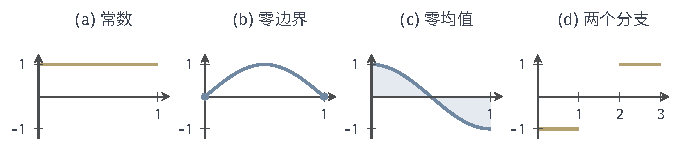
\includegraphics[width=114.4mm]{figures/02-abstract-mathematics/03-function-spaces/tikz/c4-poincare/figure.pdf}
  \caption{Poincaré不等式中约束的作用。(a)~常数$u=1$：$u'=0$而$\|u\|_{L^2}=1$，没有约束时导数控制不了函数。(b)~零边界$u=\sin(\pi x)$：$\|u\|_{L^2}/\|u'\|_{L^2}=1/\pi$。(c)~零均值$u=\cos(\pi x)$（阴影正负面积相等）：比值同为$1/\pi$。(d)~两个分支$(0,1)\cup(2,3)$上分别取$-1$与$1$：均值为零、导数为零，说明零均值形式需要区域连通。}
  \label{fig:sob-poincare}
\end{figure*}

\begin{theorem}[Poincaré不等式]
\label{thm:sob-poincare}
\begin{enumerate}
 \item 设$\Omega$为有界开集。存在常数$C$，使所有$u\in H_0^1(\Omega)$满足$\|u\|_{L^2}\le C\|\nabla u\|_{L^2}$。
 \item 设$\Omega$为有界连通Lipschitz区域，$u_\Omega=|\Omega|^{-1}\int_\Omega u\,\mathrm dx$为均值。存在常数$C$，使所有$u\in H^1(\Omega)$满足$\|u-u_\Omega\|_{L^2}\le C\|\nabla u\|_{L^2}$。
\end{enumerate}
\end{theorem}

\paragraph{区间上的直接证明}
先在区间$(a,b)$上用积分表示直接证明，$L=b-a$。对零边界情形，由$H_0^1$的定义和稠密性，只需对$u\in C_c^\infty(a,b)$证明（两边对$H^1$范数连续）。此时$u(a)=0$，$u(x)=\int_a^xu'(t)\,\mathrm dt$，由Cauchy--Schwarz不等式$|u(x)|^2\le(x-a)\|u'\|_{L^2}^2$，对$x$积分得
\[
 \|u\|_{L^2}^2\le\frac{L^2}{2}\|u'\|_{L^2}^2,\qquad\|u\|_{L^2}\le\frac{L}{\sqrt2}\|u'\|_{L^2} .
\]
对零均值情形，用连续代表，$|\tilde u(x)-\tilde u(y)|\le L^{1/2}\|u'\|_{L^2}$（式~\eqref{eq:sob-1d-holder}，$p=2$）。由于$\tilde u(x)-u_\Omega=L^{-1}\int_a^b(\tilde u(x)-\tilde u(y))\,\mathrm dy$，有$|\tilde u(x)-u_\Omega|\le L^{1/2}\|u'\|_{L^2}$，平方后对$x$积分得$\|u-u_\Omega\|_{L^2}\le L\|u'\|_{L^2}$。这两个常数都不是最优的。在$(0,1)$上，$\sin(\pi x)$与$\cos(\pi x)$分别满足零边界与零均值，比值$\|u\|_{L^2}/\|u'\|_{L^2}$都等于$1/\pi\approx0.318$（图~\ref{fig:sob-poincare}(b)(c)）；可以证明$L/\pi$就是两种情形的最优常数，而上面的直接估计给出$L/\sqrt2\approx0.707L$与$L$。

\paragraph{一般区域的反证路线}
高维没有这样简单的积分表示，但紧嵌入提供了一条反证路线。以零均值情形为例。反设不等式不成立，则对每个$n$有$u_n\in H^1(\Omega)$，$u_n$的均值为零，$\|u_n\|_{L^2}=1$，而$\|\nabla u_n\|_{L^2}<1/n$。

第一步，序列在$H^1$中有界（$\|u_n\|_{H^1}^2<1+1/n^2$），由定理~\ref{thm:sob-rellich}，有子列（仍记作$u_n$）在$L^2$中收敛到某个$u$。$L^2$收敛保持范数与均值，所以$\|u\|_{L^2}=1$，$u$的均值为零。

第二步，极限在$H^1$中取得，且梯度为零。由于$\|u_n-u_m\|_{H^1}^2=\|u_n-u_m\|_{L^2}^2+\|\nabla u_n-\nabla u_m\|_{L^2}^2$，前一项因$L^2$收敛而趋零，后一项不超过$(1/n+1/m)^2$，所以$(u_n)$是$H^1$中的Cauchy列。由定理~\ref{thm:sob-complete}，它在$H^1$中收敛，极限只能是$u$，并且$\|\nabla u\|_{L^2}=\lim\|\nabla u_n\|_{L^2}=0$。

第三步，梯度为零的函数在连通区域上是常数。由式~\eqref{eq:sob-mollifier-commute}，$\nabla(u*\rho_\varepsilon)=(\nabla u)*\rho_\varepsilon=0$在$\Omega_\varepsilon$上成立。对闭包含于$\Omega$的任一球$B$，$\varepsilon$足够小时$B\subset\Omega_\varepsilon$，光滑函数$u*\rho_\varepsilon$在连通的$B$上为常数；令$\varepsilon\to0$，由局部$L^2$恢复，$u$在$B$上几乎处处等于这些常数的极限。相交的两个球上常数相同，而连通开集中任意两点可以用有限个依次相交的球连接，所以$u$在$\Omega$上几乎处处为同一个常数。均值为零迫使这个常数为零，与$\|u\|_{L^2}=1$矛盾。

零边界情形的反证几乎相同。先说明可以只在球上讨论：取一个闭包包含$\overline\Omega$的开球$B_0$，把$H_0^1(\Omega)$的函数在$\Omega$外补成零。对$C_c^\infty(\Omega)$中的函数，零延拓属于$C_c^\infty(B_0)$，$H^1$范数不变；由闭包的定义，零延拓把$H_0^1(\Omega)$等距地映入$H_0^1(B_0)$，并且像中的函数在$B_0\setminus\Omega$上为零。于是只需对球$B_0$上、在$B_0\setminus\Omega$上为零的$H_0^1$函数证明不等式。$B_0$是连通的Lipschitz区域，第一步的紧嵌入可用；第二步的极限$u$仍属于闭子空间$H_0^1(B_0)$，在$B_0\setminus\Omega$上为零，梯度为零；第三步给出$u$在$B_0$上为常数，而$B_0\setminus\Omega$包含一个正测度的环形区域，所以常数为零，同样矛盾。这一论证不需要$\Omega$连通或有Lipschitz边界。

\paragraph{条件为什么不能少}
反证路线清楚地显示了每个条件的作用：紧嵌入把“导数趋于零”变成一个强收敛的极限；弱梯度为零只能推出“在每个连通分支上为常数”；最后由零边界或零均值把常数消去。去掉连通性，零均值不足以消去常数，图~\ref{fig:sob-poincare}(d)在$(0,1)\cup(2,3)$上取$-1$与$1$，均值为零、导数为零，不等式失败。去掉约束，常数函数本身就是反例。去掉区域有界，紧嵌入失效：在整条实轴上，$u_R(x)=\psi(x/R)$满足$\|u_R\|_{L^2}=R^{1/2}\|\psi\|_{L^2}$而$\|u_R'\|_{L^2}=R^{-1/2}\|\psi'\|_{L^2}$，比值随$R$无界，零边界也救不回来。

% 第4章第6节：本章小结。

\section{本章小结}
\label{sec:sob-summary}

本章开头的问题是：经典导数失效以后，怎样保存变化的信息，以及控制了函数和它的变化之后能得到什么。回答由一条对象链和四个分支问题组成，图~\ref{fig:sob-object-relations}把它们画在一起。

\begin{figure*}[!htb]
  \centering
  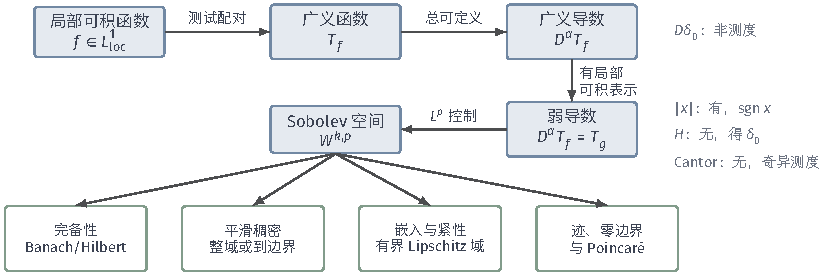
\includegraphics[width=140.6mm]{figures/02-abstract-mathematics/03-function-spaces/tikz/c4-object-relations/figure.pdf}
  \caption{本章的对象关系。上行：局部可积函数经测试配对成为广义函数，广义导数总能定义；只有当广义导数有局部可积表示时才得到弱导数，再加上$L^p$大小的控制便得到Sobolev空间。下行：Sobolev空间上分别研究的四个问题，其中嵌入、紧性与迹需要有界Lipschitz区域等条件。右侧的例子检验对象链的边界：$\delta_0$的导数不是测度，$|x|$有弱导数，阶跃与Cantor函数的广义导数分别是点质量与奇异测度。}
  \label{fig:sob-object-relations}
\end{figure*}

\paragraph{对象链及其边界}
从分部积分出发，我们把导数转移到紧支撑的光滑测试上。局部可积函数通过积分配对成为广义函数，广义导数对每个广义函数都有定义，但输出可能超出函数甚至测度的范围，$D\delta_0$就是这样。当广义导数恰好由一个局部可积函数表示时，称之为弱导数；测试函数能区分局部可积函数，所以弱导数在几乎处处意义下唯一。尖点函数$|x|$有弱导数$\operatorname{sgn}x$；阶跃函数的广义导数是$\delta_0$，Cantor函数的广义导数是集中在零测集上的奇异测度，两者都没有弱导数，尽管它们几乎处处有经典导数。在一维，弱可微恰好等价于有绝对连续代表，即能从导数积分恢复函数；导数的积分指数$p$进一步决定代表的Hölder指数$1-1/p$。把函数和直到$k$阶的弱导数的$L^p$大小同时放进范数，得到Sobolev空间$W^{k,p}$；零阶项控制水平，导数项控制变化。

\paragraph{四个问题各自的条件}
在Sobolev空间上，我们分别回答了几个不能互相代替的问题。完备性对任意开集成立，$H^k$因而是Hilbert空间，但它不提供连续代表、边界值或强收敛子列。光滑逼近分三层：磨光与弱导数交换给出局部逼近；单位分解把它拼成任意开集上的内部光滑逼近；光滑到边界的逼近需要Lipschitz边界和延拓。连续嵌入由积分指数与维数比较决定：$p<d$时得到$L^{p^*}$，$p>d$时得到Hölder连续代表，临界的$p=d\ge2$两者都差一点；缩放论证解释了$p^*=dp/(d-p)$的来源，幂函数检验了它的精确性。紧嵌入在有界Lipschitz区域上把有界序列变成$L^q$（$q<p^*$）中收敛的子列，在临界指数处因集中而失效，在无界区域上因平移逃逸而失效。边界迹把光滑函数的边界限制延拓为$H^1(\Omega)\to L^2(\partial\Omega)$的有界算子，输出是边界上的等价类；零迹函数恰好构成$H_0^1$。Poincaré不等式在排除常数方向之后，让导数单独控制函数，零边界与零均值是两种排除方式，后者还需要区域连通。

\paragraph{与后续内容的关系}
这些空间和工具为后面的问题提供了语言。第~\ref{chap:rkhs}章研究点值读取连续的Hilbert函数空间，本章一维的端点估计和$H^k$（$k>d/2$）的连续代表是那里的具体例子，而高维$H^1$在一点附近可以无界，则说明点值连续并非理所当然。在优化中，Sobolev空间用来指定目标函数的定义域，$G+H_0^1$给出保持边界值的可行扰动，紧嵌入配合弱收敛子列处理极小化序列；在微分方程与演化问题中，它们用来表达弱解。本章只建立空间、微分和边界的工具，不由这些工具直接断言某个具体问题有解。

